\documentclass[12pt,a4paper]{report}
\usepackage[utf8]{inputenc}
\usepackage[sfdefault]{ClearSans}
\usepackage[T1]{fontenc}
\usepackage[left=35mm,right=20mm,top=25mm,bottom=25mm]{geometry}
\usepackage[dvipsnames]{xcolor}
\usepackage[czech]{babel}
\usepackage{titling}
\usepackage{graphicx}
\usepackage{caption}
\usepackage[list=true]{subcaption}
\usepackage{acronym}
\usepackage{setspace}
\usepackage{indentfirst}
\usepackage{hyperref}
\usepackage{tabularx}
\usepackage{changepage}
\usepackage{tocloft}
\usepackage{array}
\usepackage{multirow}
\usepackage{listings}
\usepackage{tcolorbox}
\tcbuselibrary{listings,skins}  

% Colors
\definecolor{pojblue}{RGB}{31, 91, 157}

\definecolor{bashBackcolor}{RGB}{237, 237, 237}
\definecolor{bashKeyword}{RGB}{35, 83, 173}

% Styles
\lstdefinestyle{codeblock}{
     basicstyle=\sffamily\footnotesize\color{Black},
     keywordstyle=\color{bashKeyword},
     morekeywords={useradd, passwd, usermod, sudo, su, apt-get, wget, sh, git,node, npm, systemctl, cd, ls},
}


\usepackage{titlesec}
\titleformat{\chapter}
  {\normalfont\LARGE\bfseries}{\thechapter}{1em}{}
\titlespacing*{\chapter}{0pt}{3.5ex plus 1ex minus .2ex}{2.3ex plus .2ex}

\graphicspath{ {./img/} }
\setlength{\parindent}{2em}
\setlength{\parskip}{0.1em}
\linespread{1.5}

\renewcommand\cftchapdotsep{\cftdotsep}
\renewcommand\cftchapleader{\cftdotfill{\cftchapdotsep}}

\setcounter{secnumdepth}{5}

\title{Fotografický web a kompletní administrační systém}
\author{Jiří Vala}
\date{}

\begin{document}
\renewcommand*\listfigurename{}
\renewcommand{\figurename}{Obr.}
\renewcommand\refname{}

\newtcblisting{bash}{
      enhanced,                             %%% needed for shadow
      arc=1mm,
      top=0mm,
      bottom=0mm,
      left=0mm,
      right=0mm,
      boxrule=0pt,
      colback=bashBackcolor,
      colframe=bashBackcolor,
      coltext=black,
      listing only,
      listing options={style=codeblock}
}


\begin{titlepage}
  \begin{adjustwidth}{-20mm}{-7.5mm} 
		\vspace*{-1.5cm}
		\noindent
\includegraphics[width=\linewidth]{header.png}
	\end{adjustwidth}
	\begin{center}
		\vspace*{0.2cm}
    \color{pojblue}
		\Huge\textbf{MATURITNÍ ZKOUŠKA}
    \color{black}
    \vspace*{1cm} \\
		\large \emph{PRAKTICKÁ ZKOUŠKA Z ODBORNÝCH PŘEDMĚTŮ}
		\vspace*{1cm} \\
		\Large Téma č.3 \\
		\vspace*{1cm}
		\Large Fotografický web a kompletní administrační systém \\
		\vfill
		\normalsize
	\end{center}
	\begin{tabularx}{\textwidth}{l@{\hskip 0.5cm}XXl}
		Obor vzdělání: & \multicolumn{3}{c}{\textbf{18 – 20 – M/01 Informační technologie}} \\[10pt]
		Třída: & \textbf{4. IT} & Autor práce: & \textbf{Jiří Vala} \\[10pt]
		Školní rok: & \textbf{2021/22} & Vedoucí učitel práce: & \textbf{Ing. Jiří Sumbal}
		\vspace*{1cm}
	\end{tabularx}
\end{titlepage}

\section*{Prohlášení Autora}
  „Prohlašuji, že jsem tuto práci vypracoval samostatně a použil jsem literárních pramenů a informací, které cituji a uvádím v seznamu použité literatury a dalších zdrojů informací.“ \\
	\vspace*{0.5cm} \\
	\renewcommand{\arraystretch}{2}
	\begin{tabularx}{\textwidth}{l@{\hskip 0.75cm}X@{\hskip 1.5cm}X@{\hskip 0.75cm}l}
		Ve Frýdku-Místku, dne: & \dotfill & \dotfill & podpis \\
	\end{tabularx}
  \clearpage

  \section*{Anotace}
  Tato práce se zabývá průběhem vývoje webové stránky pro amatérského 
  fotografa ve formě virtuální galerie a jejího administračního systému.
  Popisuje použité technologie a postupy ve vývoji spolu s konfigurací
  jednotlivých služeb klíčových ke spuštění celého projektu
  na produkční server a jeho správné a dlouhodobě nezávadné fungování.
  
  \section*{Anotation}
  This thesis focuses on the development process\dots \\TODO!

  \section*{Klíčová slova}
  
  \noindent webová stránka; webová aplikace; administační systém; webová prezentace; webová galerie; vývoj; javascript; react; linux; webhosting
  
  \clearpage
  
  \tableofcontents
  
  \clearpage

  \chapter{Vymezení pojmů}
  \begin{enumerate}
    \item \textbf{Content Management System} - Administrační systém, je systém, který umožňuje manipulaci s daty a obsahem webové stránky či webové (ale i desktopové) aplikace. 
    \item \textbf{Hosting (Webhosting)} - Znamená pronájem prostoru na cizím webovém serveru za účelem spuštění webové stránky či aplikace. 
    \item \textbf{Continuous Deployment (CI/CD)} - CI - Continuous Intergration a CD - Continuous Delivery je proces, který umožňuje nepřetržité dodávání aktuální verze projektu k testování či produkčnímu spuštění. V praxi to znamená, že pokud tým vývojářů provede změnu a uloží ji do remote repositáře (místo pro ukládání zdrojových kódů v cloudu), tato změna se automaticky projeví (deployne) na produkční server (server, na kterém je spuštěna aktuální verze projektu a je poskytována uživatelům z venčí).
    \item \textbf{Fetching} - Proces během kterého se "stahují" data z databáze. Tento anglický výraz doslova znamená "přinést".
    \item \textbf{Backend(Server)} -  Logická část aplikace nebo webu. Požadavky, které uživatel aplikace provede (například přejmenování záznamu v databázi) a data (například všechny záznamy), které si vyžádá, tento server nejdříve zpracuje, případně vytáhne z databáze a pak je odešle uživateli aplikace, která je následně zobrazí, či případně upraví v databázi.
    \item \textbf{Frontend} - Jedná se o grafické uživatelské rozhraní, v rámci webových aplikací a stránek většinou nejčastěji pomocí značkovacího jazyka HTML, stylovacího jazyka CSS a scriptovacího jazyka Javascript.
    \item \textbf{Cloud Computing Provider} - Poskytovatel cloudových služeb a infrastruktury (serverů).
    \item \textbf{Public/Private API} - API je soubor procedur, funkcí a protokolů zajišťující komunikaci mezi dvěma platformami, které si vzájemně vyměňují data (například dvě rozdílné aplikace). K public API má přístup kdokoliv, k private API jen autentifikovaní uživatele například pomocí unikátního ID tokenu.
    \item \textbf{DDOS útok} - Distributed Denial Of Service - je útok jehož cílem je pomocí sítě mnoha virtuálních počítačů, které v jednu chvíli budou provádět požadavky na daný server, vyřadit tento server z provozu, jelikož nezvládne nápor takového počtu požadavků a zhroutí se.
    \item \textbf{Framework} - Jedná se o podpůrnou softwarovou strukturu, která zjednodušuje vývoj a organizaci projektu v daném jazyce. Může obsahovat další funkce, podpůrné programy nebo vzory a doporučené postupy ve vývoji.
    \item \textbf{Knihovna} - Jedná se souhrn procedur a funkcí, často avšak také konstant a datových typů, které usnadňují vývojáři práci tím, že může použít již hotový kód.
    \item \textbf{Open-source} - Jedná se o projekt s otevřeným zdrojovým kódem, což znamená, že na jeho vývoji se může podílet každý a každý si jej může stáhnout. Popularita open-source projektů v posledních letech velmi roste.
    \item \textbf{CRUD operace} - Create, read, update, delete (vytvořit, číst, změnit, smazat) jsou čtyři základní operace se záznamem v databázové tabulce.
    \item \textbf{Shell} - Jedná se o vrstvu operačního systému, která provádí příkazy a spouští programy.
    \item \textbf{Pagination} - Jedná se o proces rozdělování obsahu na jednotlivé stránky a podstránky. Nejčastěji ji vidíme ve formě čísel na konci webové stránky.
    \item \textbf{Dropdown menu} -  Jedná se o list záznamů, který se zobrazí až ve chvíli, kdy uživatel nějakým způsobem provede interakci s tímto menu, například kliknutím myši.
    \item \textbf{Algoritmus} - Proces jednotlivých příkazů za účelem splnění zadaného úkolu.
    \item \textbf{Push notifikace} - Notifikace, které se zobrazují uživateli na mobilním zařízení v notifikační listě nebo na zamykací obrazovce.
  \end{enumerate}
  \section{Seznam použítých zkratek}
  \begin{enumerate}
    \item \textbf{DMP} - Dlouhodobá maturitní práce
    \item \textbf{CMS} - Content Management System
    \item \textbf{VPS} - Virtual Private Server
    \item \textbf{CI} - Continuous Integratiaon
    \item \textbf{CD} - Continuous Deployment
    \item \textbf{API} - Application Programming Interface
    \item \textbf{GNU} - GNU's Not Unix
    \item \textbf{ISO} - 
    \item \textbf{GUI} - Graphical User Interface
    \item \textbf{CLI} - Command Line Interface
    \item \textbf{UI/UX} - User Interface/User Experience
  
  \end{enumerate} 
  
  \chapter{Zadání práce}
  Pan Milan Bureš st. (dále jen fotograf nebo zákazník) je amatérský fotograf, který si již před pár lety
  nechal na zakázku vytvořit webovou stránku, na které by prezentoval své fotografie, zachycující
  náhodné okamžiky jeho života. Nicméně postupem času se jeho web i administrační systém stali
  zastaralými a bylo potřeba celý systém zmodernizovat i vzhledem k faktu, že jeho webová stránka
  fungovala pomocí Adobe Flash Player, kterému skončila podpora a není již podporovaný
  moderními prohlížeči.
  Proto mě v rámci dlouhodobé maturitní práce zprostředkované mým garantem kontaktoval a
  požádal, zda-li bych jeho webovou prezentaci nemohl modernizovat. Mým úkolem bylo vytvořit
  web, který bude sloužit jako virtuální galerie jeho fotografií a bude zobrazitelná a funkční na všech
  zařízeních, a administrační systém (dále jen CMS), který bude umožňovat nahrávání, správu a
  manipulaci fotografií či alb, ve kterých se jednotlivé fotografie seskupují.
  Pro potřeby mé maturitní práce bylo potřeba, aby projekt obsahoval i část jiného předmětu, než
  jen programování (celý systém jsem naprogramoval) a databáze (data a fotografie, které fotograf
  nahraje/uloží). Rozhodl jsem se tedy, že si vytvořím vlastní server běžící na operačním systému
  Linux, na kterém budu hostovat vlastní instanci celého systému a bude obsahovat funkcionalitu
  tzv. Continuous Deploymentu, což přesně kopíruje funkcionality komerční instance projektu určené
  jen pro účely zákazníka.


  \chapter{Klíčové vlastnosti a požadavky projektu}
  Během vývoje webové prezentace byl velký důraz kladen na to, aby se co nejvíce podobala
  stávající verzi. Ne veškeré elementy webu byly replikovatelné a také jsem se chtěl co nejvíce řídit
  pravidly dobrého webu. Pro porovnání, zde jsou screenshoty jednotlivých webových stránek.
  
  \vspace*{0.5cm}
  \noindent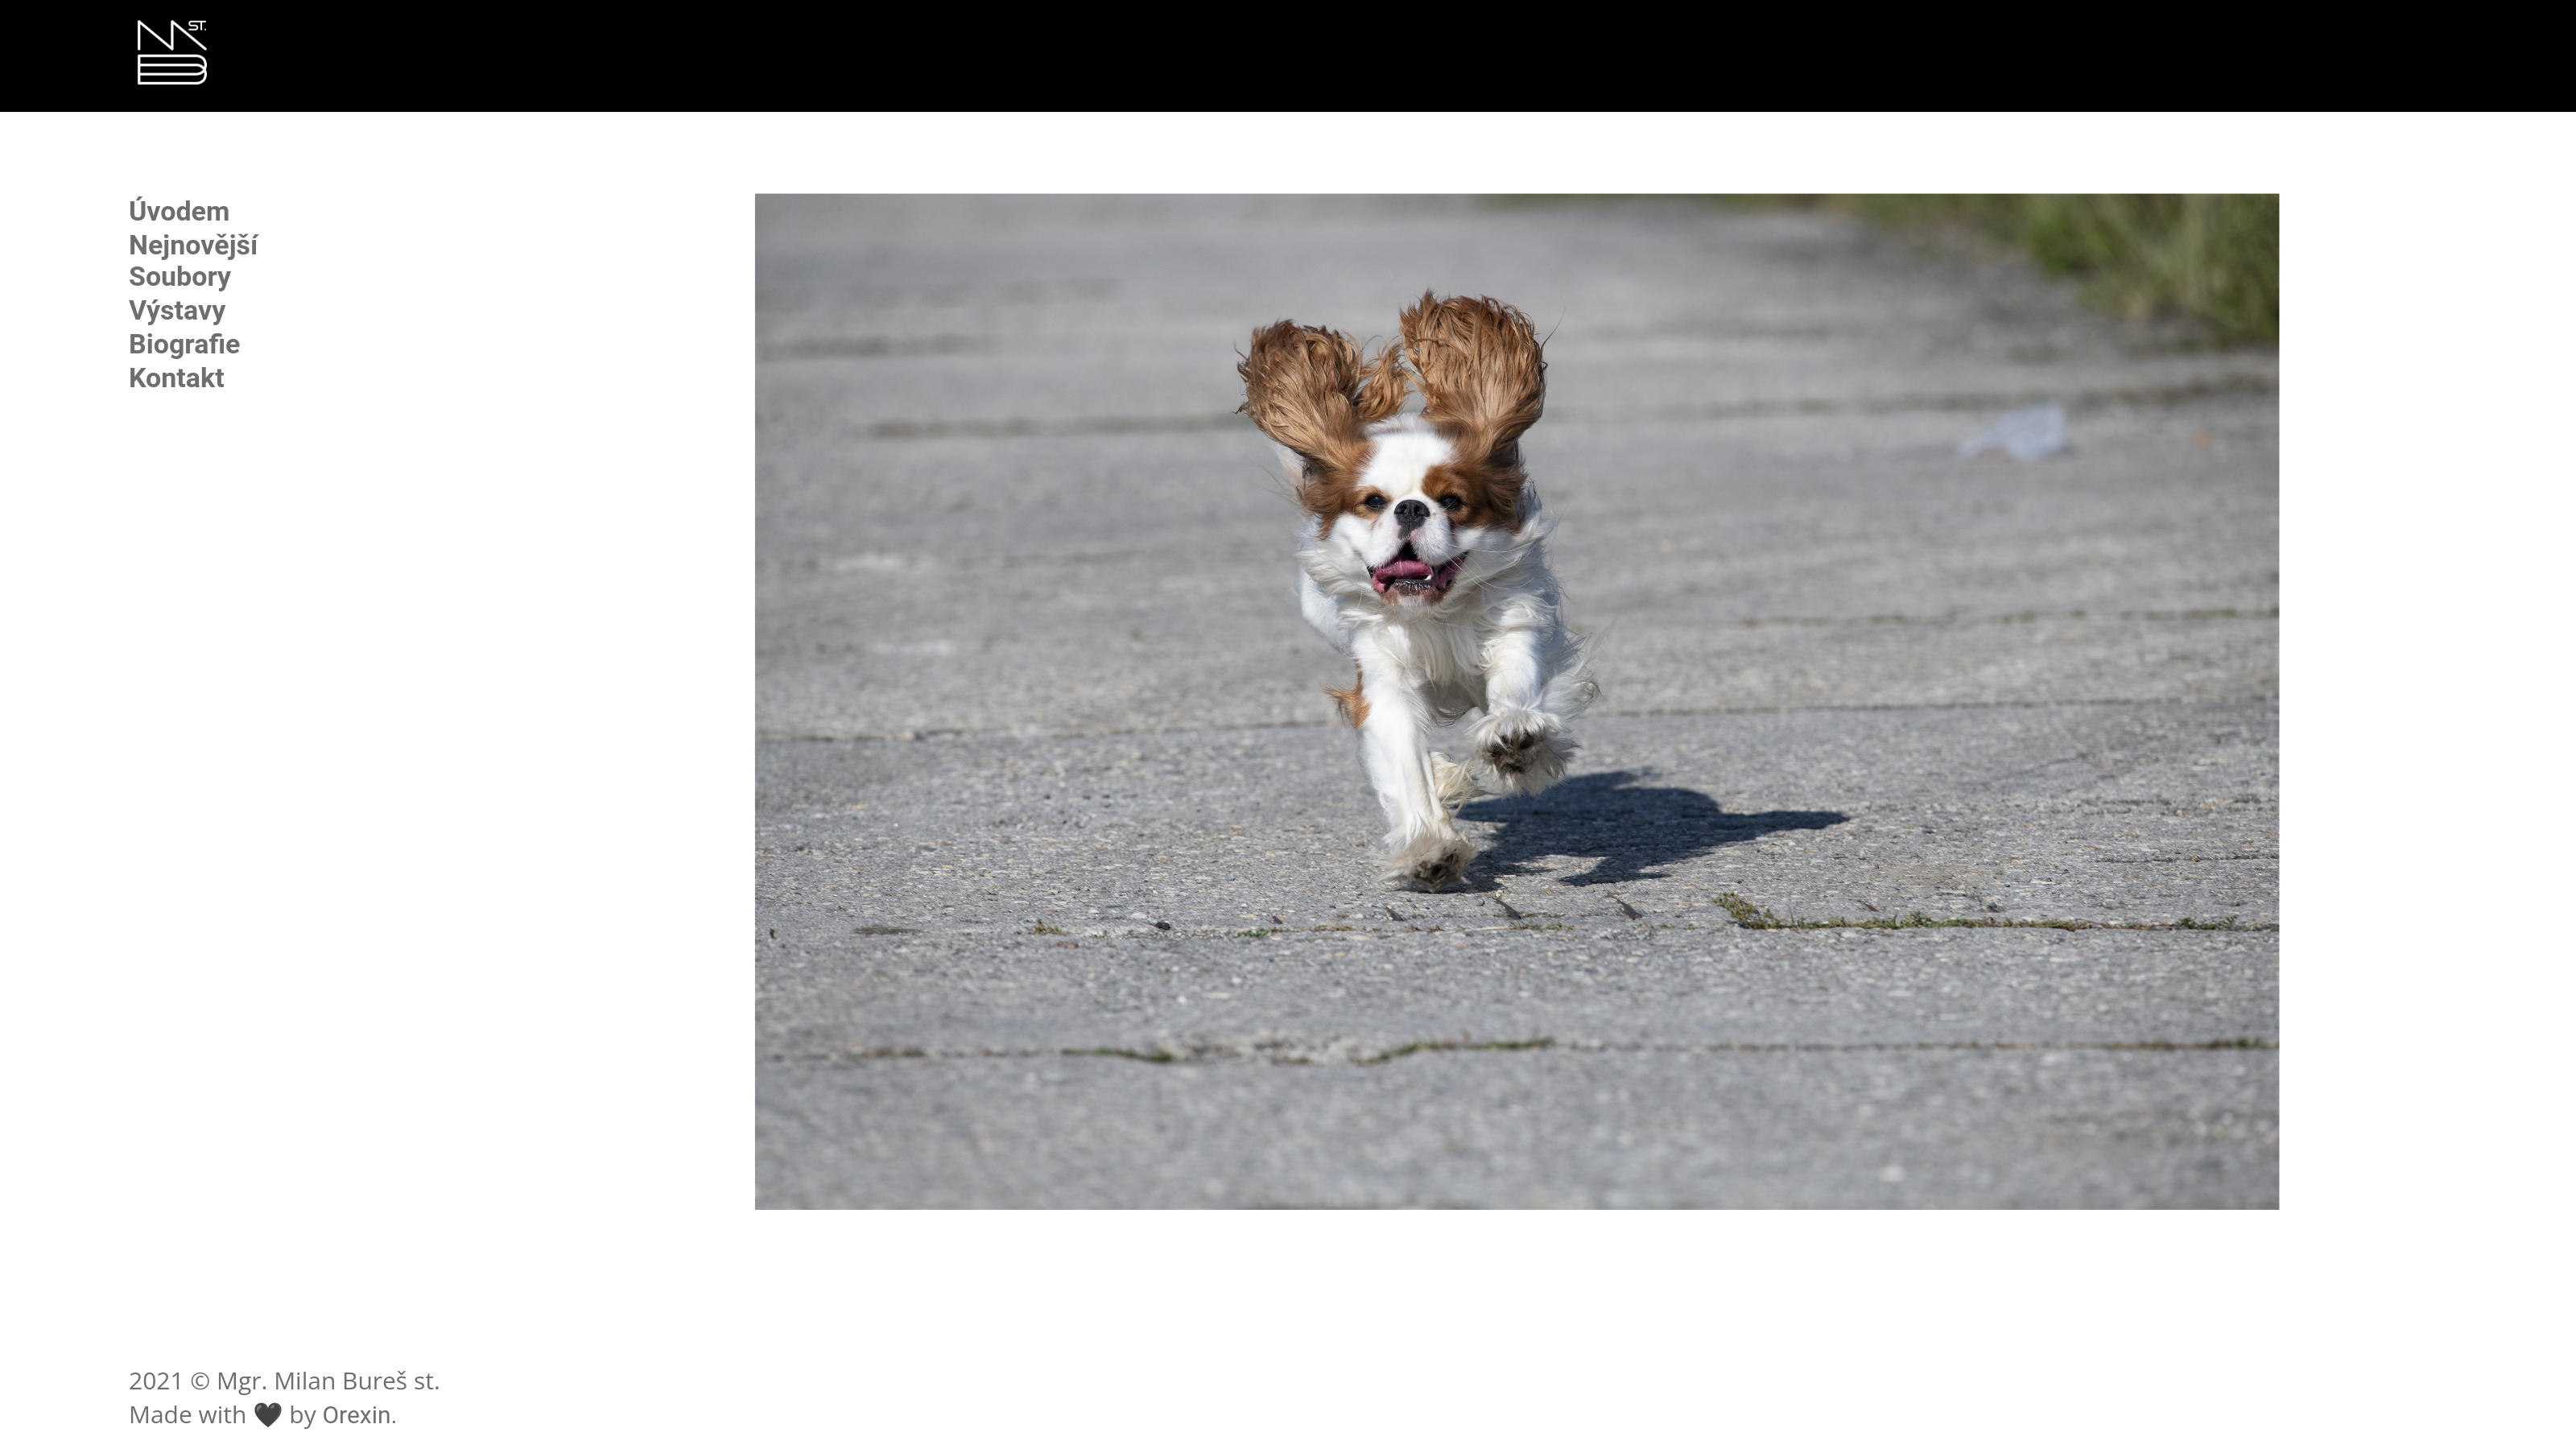
\includegraphics[width=\linewidth]{dmp-bures.png}
  \begin{center}
    Popis
  \end{center}
  \vspace*{0.5cm}
  \noindent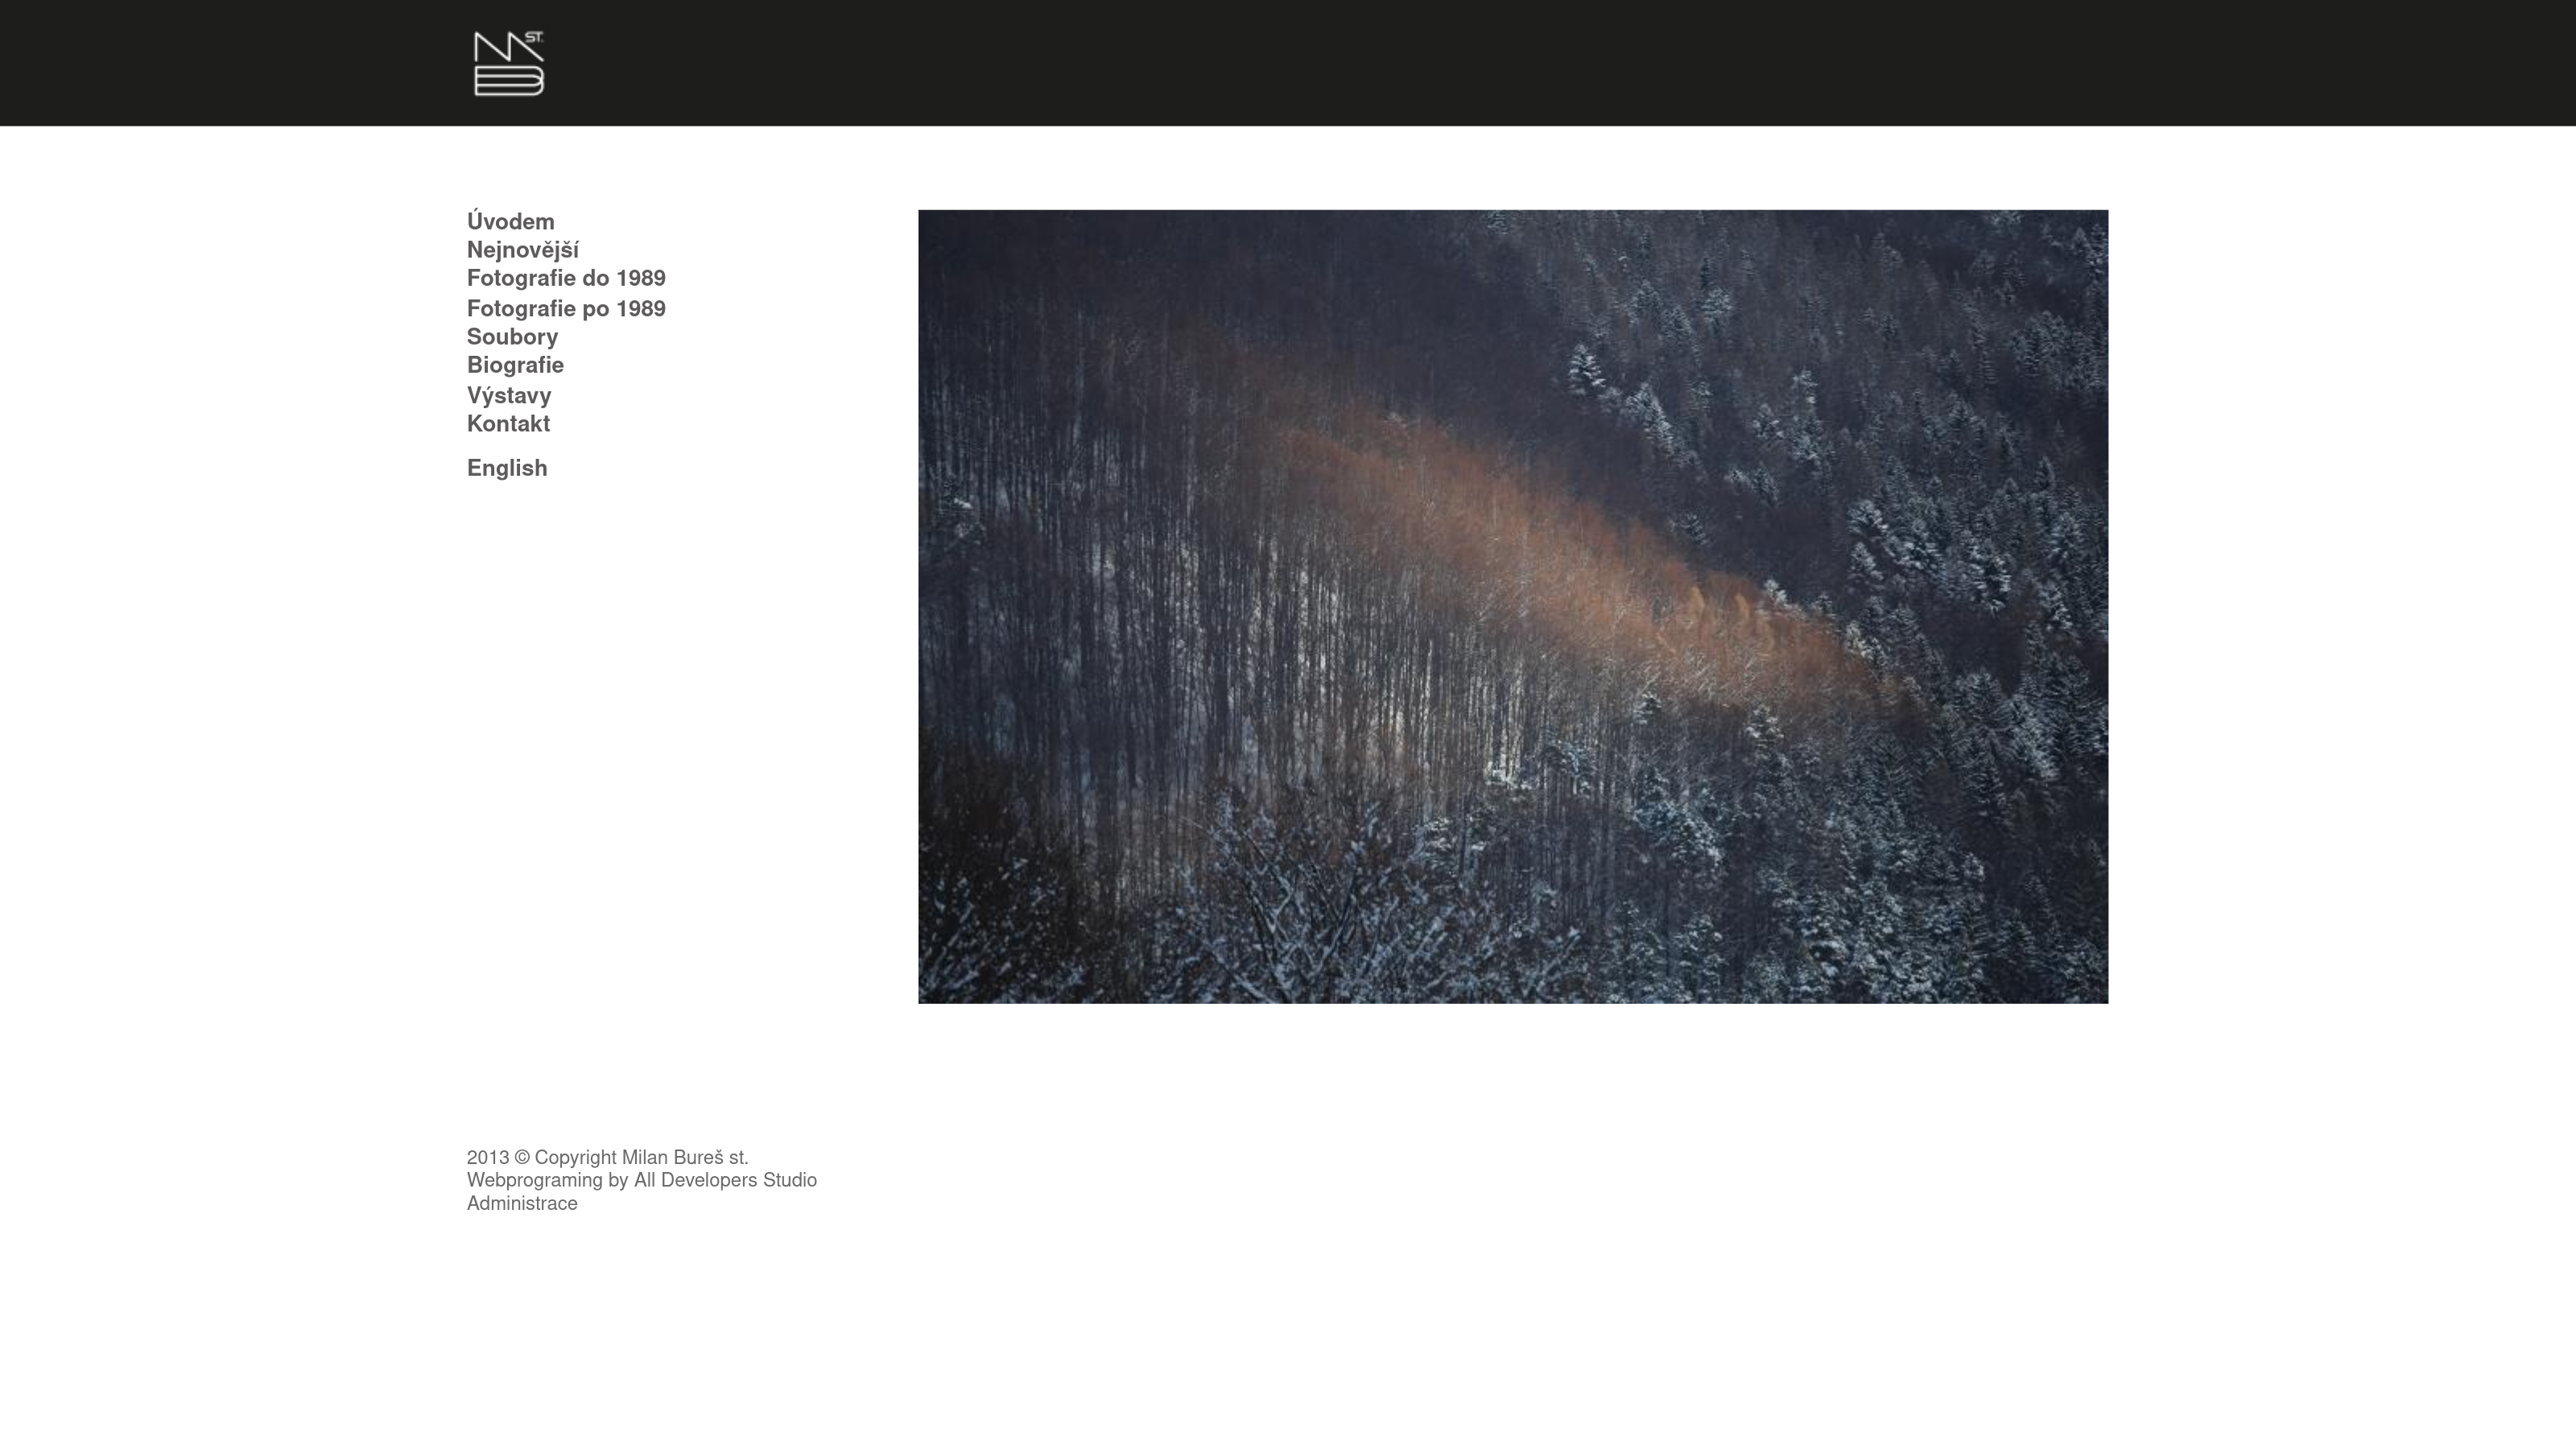
\includegraphics[width=\linewidth]{milanburescz.png}
  \begin{center}
    Popis
  \end{center}
  \vspace*{0.5cm}

  \section{Serverless architektura}
  Ačkoliv je samozřejmostí, že je jak webová prezentace tak CMS hostovaná na nějakém fyzickém
  serveru, k požadavkům jako fetching dat z databáze nepoužívám žádný další (backend) server. To
  znamená, že jsem sice odkázaný kompletně na svého cloud computing providera, což je v mém
  případě Firebase od Google, ale na druhou stranu se nemusím (a ani zákazník) starat o údržbu
  vlastního serveru a ani jeho prvotní konfiguraci, vše je tzv. out-of-the-box připravené k použití.
  Díky serverless architektuře jsem nemusel vytvářet žádný backend server s private API, pomocí
  kterého bych dostával data z databáze a cloud storage do webové prezentace nebo
  administračního systému.
  Serverless architektura má mnoho výhod, jedna z těch hlavních a největších je samozřejmě
  absence potřeby konfigurovat a později spravovat vlastní server, jelikož to kompletně
  zprostředkovává daný cloud computing provider, ale také celková cena "pronájmu" , jelikož ta se
  počítá podle počtu požadavků na danou službu (napříkad fetchování dat z databáze), bezpečnost,
  jelikož jsou tyto architektury zabezpečené například proti DDOS útokům, ale také celková
  škálovatelnost celého systému. Cloud computing provider automaticky škáluje prostředky (úložistě,
  výpočetní výkon apod.), které jsou k dispozici pro daný systém.

  \vspace*{0.5cm}
  \noindent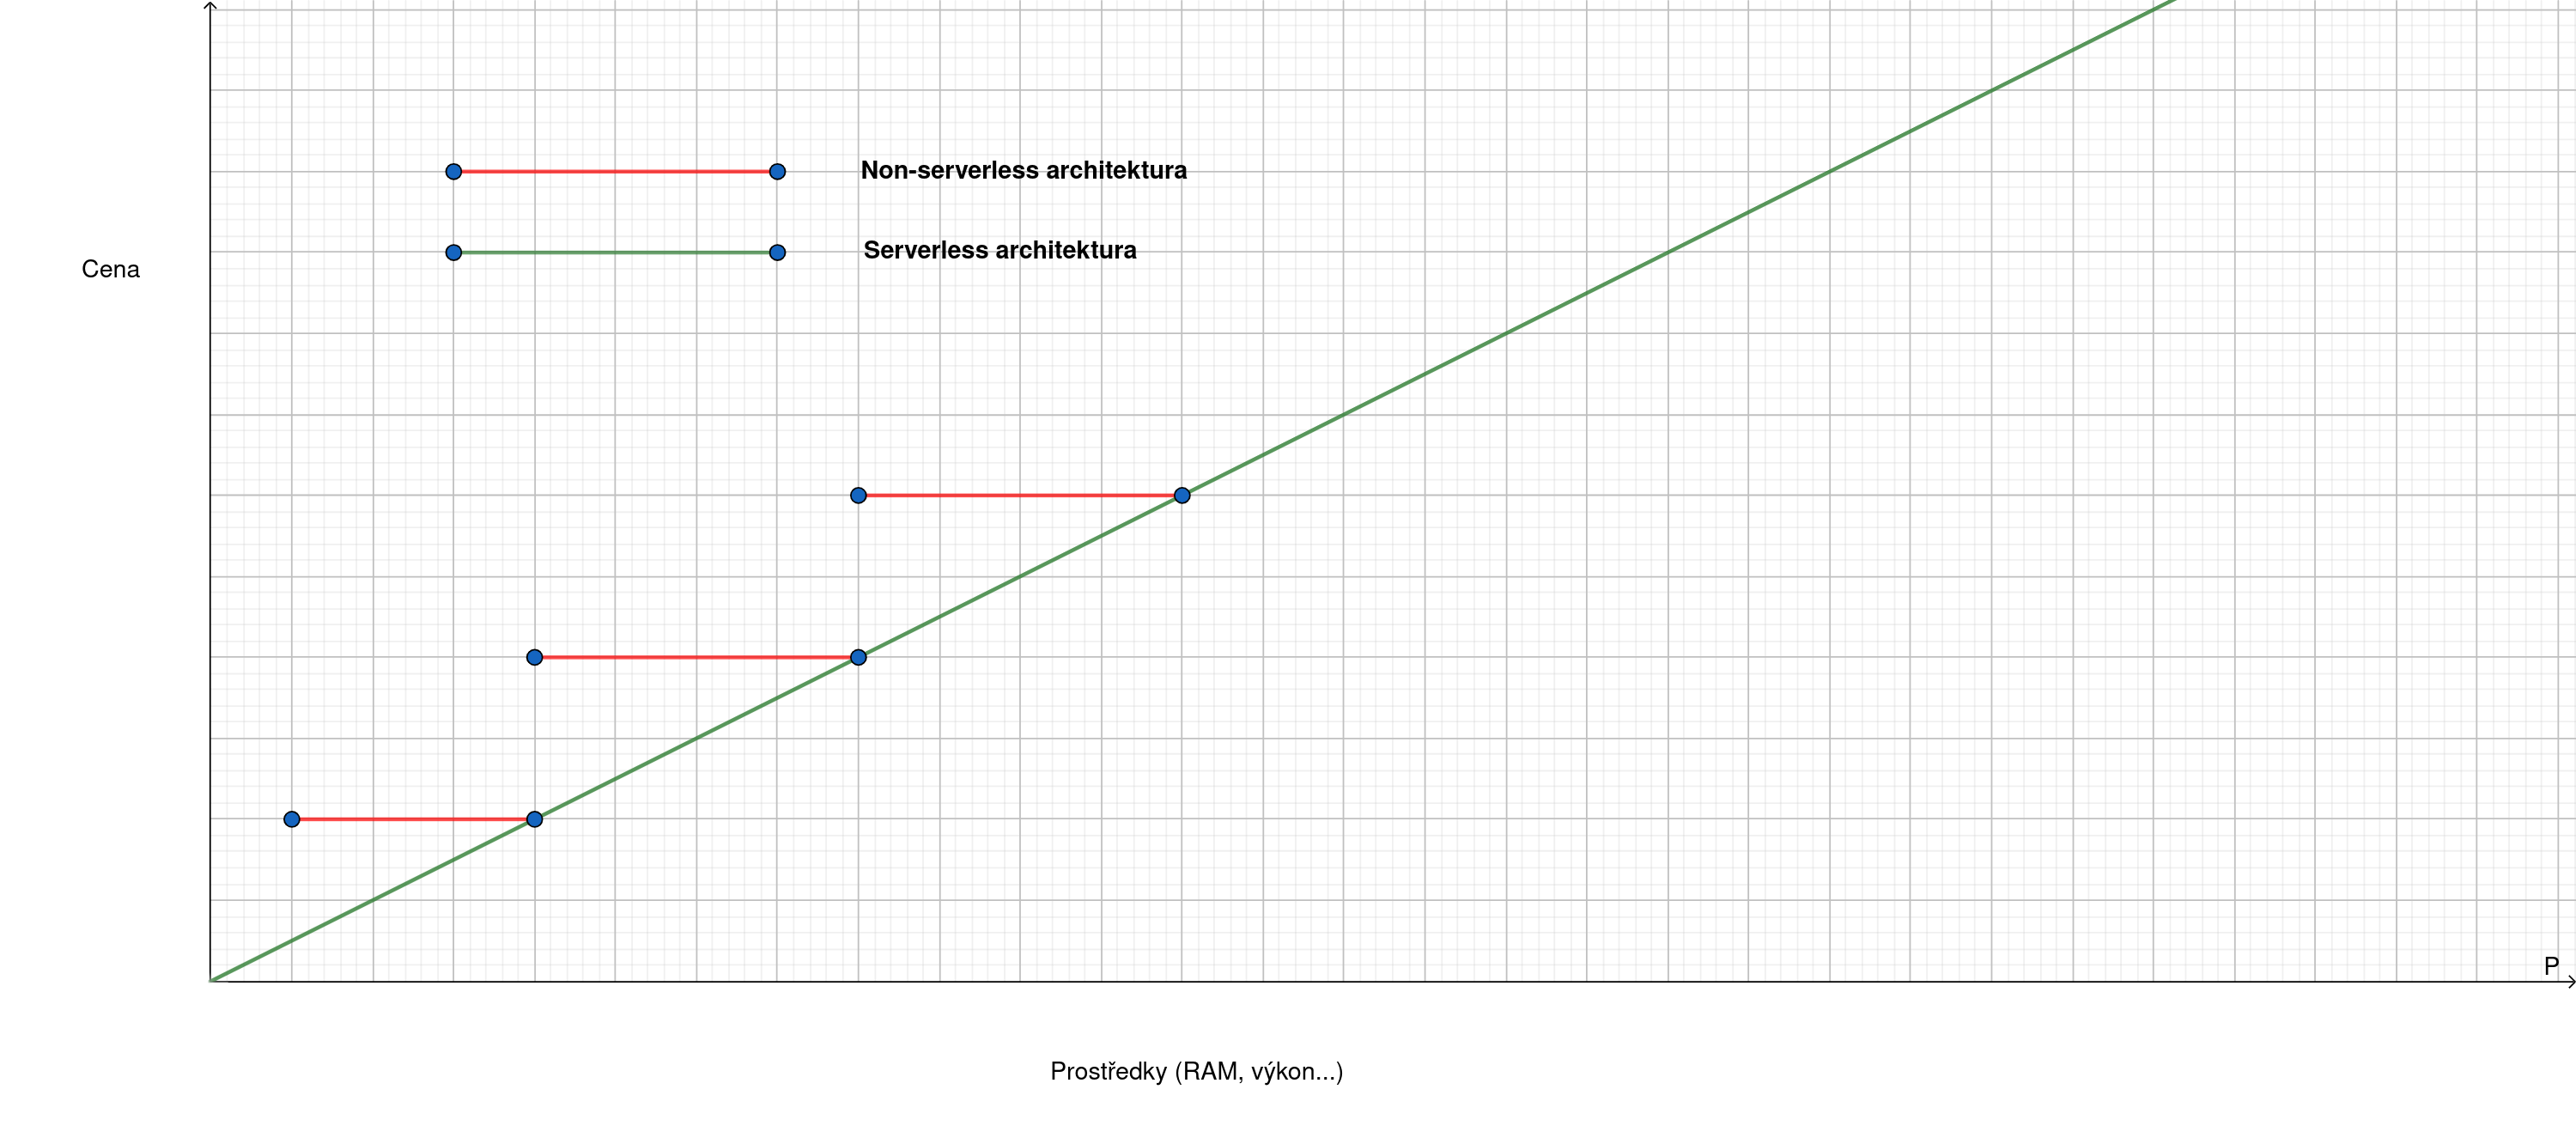
\includegraphics[width=\linewidth]{non-vs-serverless.png}
  \begin{center}
    Popis
  \end{center}
  \vspace*{0.5cm}
  Na grafu jde vidět, že pokud si zvolíme cestu non-serverless architektury, musíme s narůstajícími
  požadavky výkon zvyšovat, což ale v praxi znamená dočasné odstavení systému od provozu a
  dodatečnou správu hardwaru a tento výpočetní výkon se nemění, pokud se opět nevylepší,
  zatímco serverless řešení se automaticky škáluje.
  
  \section{Moderní technologie}
  Jelikož byla původní webová stránka i administrační systém postavena na poměrně zastaralých
  technologiích, bylo potřeba modernizovat a během vývoje jsem používal jen ty nejmodernější a
  mezi vývojáři velmi rozšířené technologie.
  \subsection{Frontend a UI/UX}
  Jedná se o grafické uživatelské rozhraní, v rámci webových aplikací většinou nejčastěji pomocí
  značkovacího jazyka HTML, stylovacího jazyka CSS a scriptovacího jazyka Javascript. Nicméně v
  dnešní době na tyto technologie, které existují delší dobu, existuje mnoho frameworků a knihoven,
  které nejen zjednodušují práci vývojářům, ale také celkově zlepšují performance aplikace či webu,
  která je díky tomu rychlejší, intuitivnější a použitelnější, což ve výsledku znamená, že například
  návštěvník webové stránky neztratí zájem, jelikož se stránka nebude dlouze načítat.
  UI (user interface - uživatelské prostředí) a UX (user experience - v hrubém překladu uživatelská
  zkušenost) je sada pravidel a procedur, kterém mají za úkol zjednodušit uživatelskou interakci se
  systémem tak, aby se uživateli produkt používal co nejsnáze a byl co nejvíce intuitivní. Během
  vývoje administračního systému jsem se inspiroval návrhem, který jsem našel na designovém
  webu Dribble.com.
  \subsubsection{HTML,CSS a Javascript}
  Jedná se o základní technologie, se kterými se dnes vyvíjejí webové stránky či aplikace a všechny
  ostatní technologie si z nich něco vzaly.
  Základním stavebním kamenem webové stránky i aplikace je HTML dokument, který obsahuje
  všechny elementy, které má web zobrazovat.
  Tyto elementy nastyluje stylovací jazyk CSS, což znamená, že v CSS dokumentu vybereme
  jednotlivý HTML element pomocí CSS selektoru a nastavíme mu například jinou barvu, šířku, či
  například nastavíme animaci, která se spustí po tom, co uživatel přes tento element přejede myší.
  Pokud má mít web nějakou funkcionalitu, například po zadaní dvou čísel vypočítat součet,
  použijeme Javacript. Ten je vlastně logickým mozkem celého webu a stará se o tyto početní
  operace, získávání dat z databáze a jejich následné vložení do struktury HTML dokumentu (DOM)
  nebo interaktivitu s uživatelem.
  \subsubsection{React.js}
  React.js je Javascriptový framework vyvíjený firmou Meta (Facebook) a open-source komunitou
  vývojářů po celém světě a k dnešnímu dni se jedná o nejvíce používaný framework na světě pro
  jeho jednoduchost a modularitu.
  Je optimální pro tvorby SPA (single page aplikací), jako je například administrační systém, protože
  velmi dobře pracuje s rychle měnícími se daty. Během vývoje react aplikace se celá aplikace
  rozdělí na jednotlivé komponenty, což má za následek jednoduchý a přehledný zdrojový kód a
  celou strukturu projektu, což je potřebné u velkého a komplexního projektu a já sám jsem během
  vývoje pocítil výrazný rozdíl v jednoduchosti vývoje oproti samotného vanilla Javascriptu (bez
  použití frameworku či knihovny.)

  [react codeblock]
  \subsubsection{SASS/SCSS}
  SASS je preprocessor stylovacího jazyka CSS, což znamená, že styly psané v SCSS (sassy css)
  zpracuje a překompiluje to klasického CSS.
  SCSS je další z mnoha stylovacích jazyků a jedná se o přímé rozšíření klasického CSS, přidává
  například proměnné, nesting, což znamená, že jednotlivé selektory můžeme psát přímo
  hierarchicky do sebe a pod sebe, což zlepšuje přehlednost jednotlivých stylů a například tzv.
  mixins, což jsou vlastně bloky stylů, které se dají použít vícekrát, což snižuje počet stylů, které musí
  vývojář napsat.

  [css codeblock]

  [scss codeblock]
  \section{Backend}
  \subsubsection{Node.js}
  Node.js je tzv. runtime pro Javascript určený k vytváření vysoce škálovatelných backend aplikací a
  webových serverů. Toto má společné např. s jazykem PHP, který má stejné zaměření. JavaScript se
  tedy díky tomuto prostředí dá používat i na serveru a ne jen na druhém konci, u klienta. Avšak na
  rozdíl např. od zmíněného PHP je v Node.js kladen důraz na vysokou škálovatelnost, tzn.
  schopnost obsloužit mnoho připojených klientů naráz. Pro tuto vlastnost a vysokou výkonnost je
  dnes Node.js velmi oblíbený pro tvorbu tzv. API serverů pro klientské single page aplikace rovněž v
  Javascriptu. 
  \subsubsection{Shell scripty}
  Shell scripty jsou sada příkazů, které po spuštění zpracovává a provede shell. Význam těchto
  scriptů v rámci tohoto projektu jsou CI/CD a DevOps Operace, které jsou detailněji popsány v bodu
  ????
  \subsubsection{Firebase}
  Firebase je cloud computing provider nabízející služby jako hosting webových stránek, hosting
  databází, ale mnoho dalších jako je například machine learning, které však pro mě vzhledem k
  povaze projektu nejsou důležité. V tomto projektu zajišťuje všechny tyto zmíněné služby a nebýt
  Firebase, musel bych je všechny řešit sám, například pronájmem dalšího serveru, kde by byly
  databáze a podobně.
  Databáze, které v rámci Firebase využívám, jsou tzv. Firestore a Cloud Storage.

  \vspace*{0.5cm}
  \noindent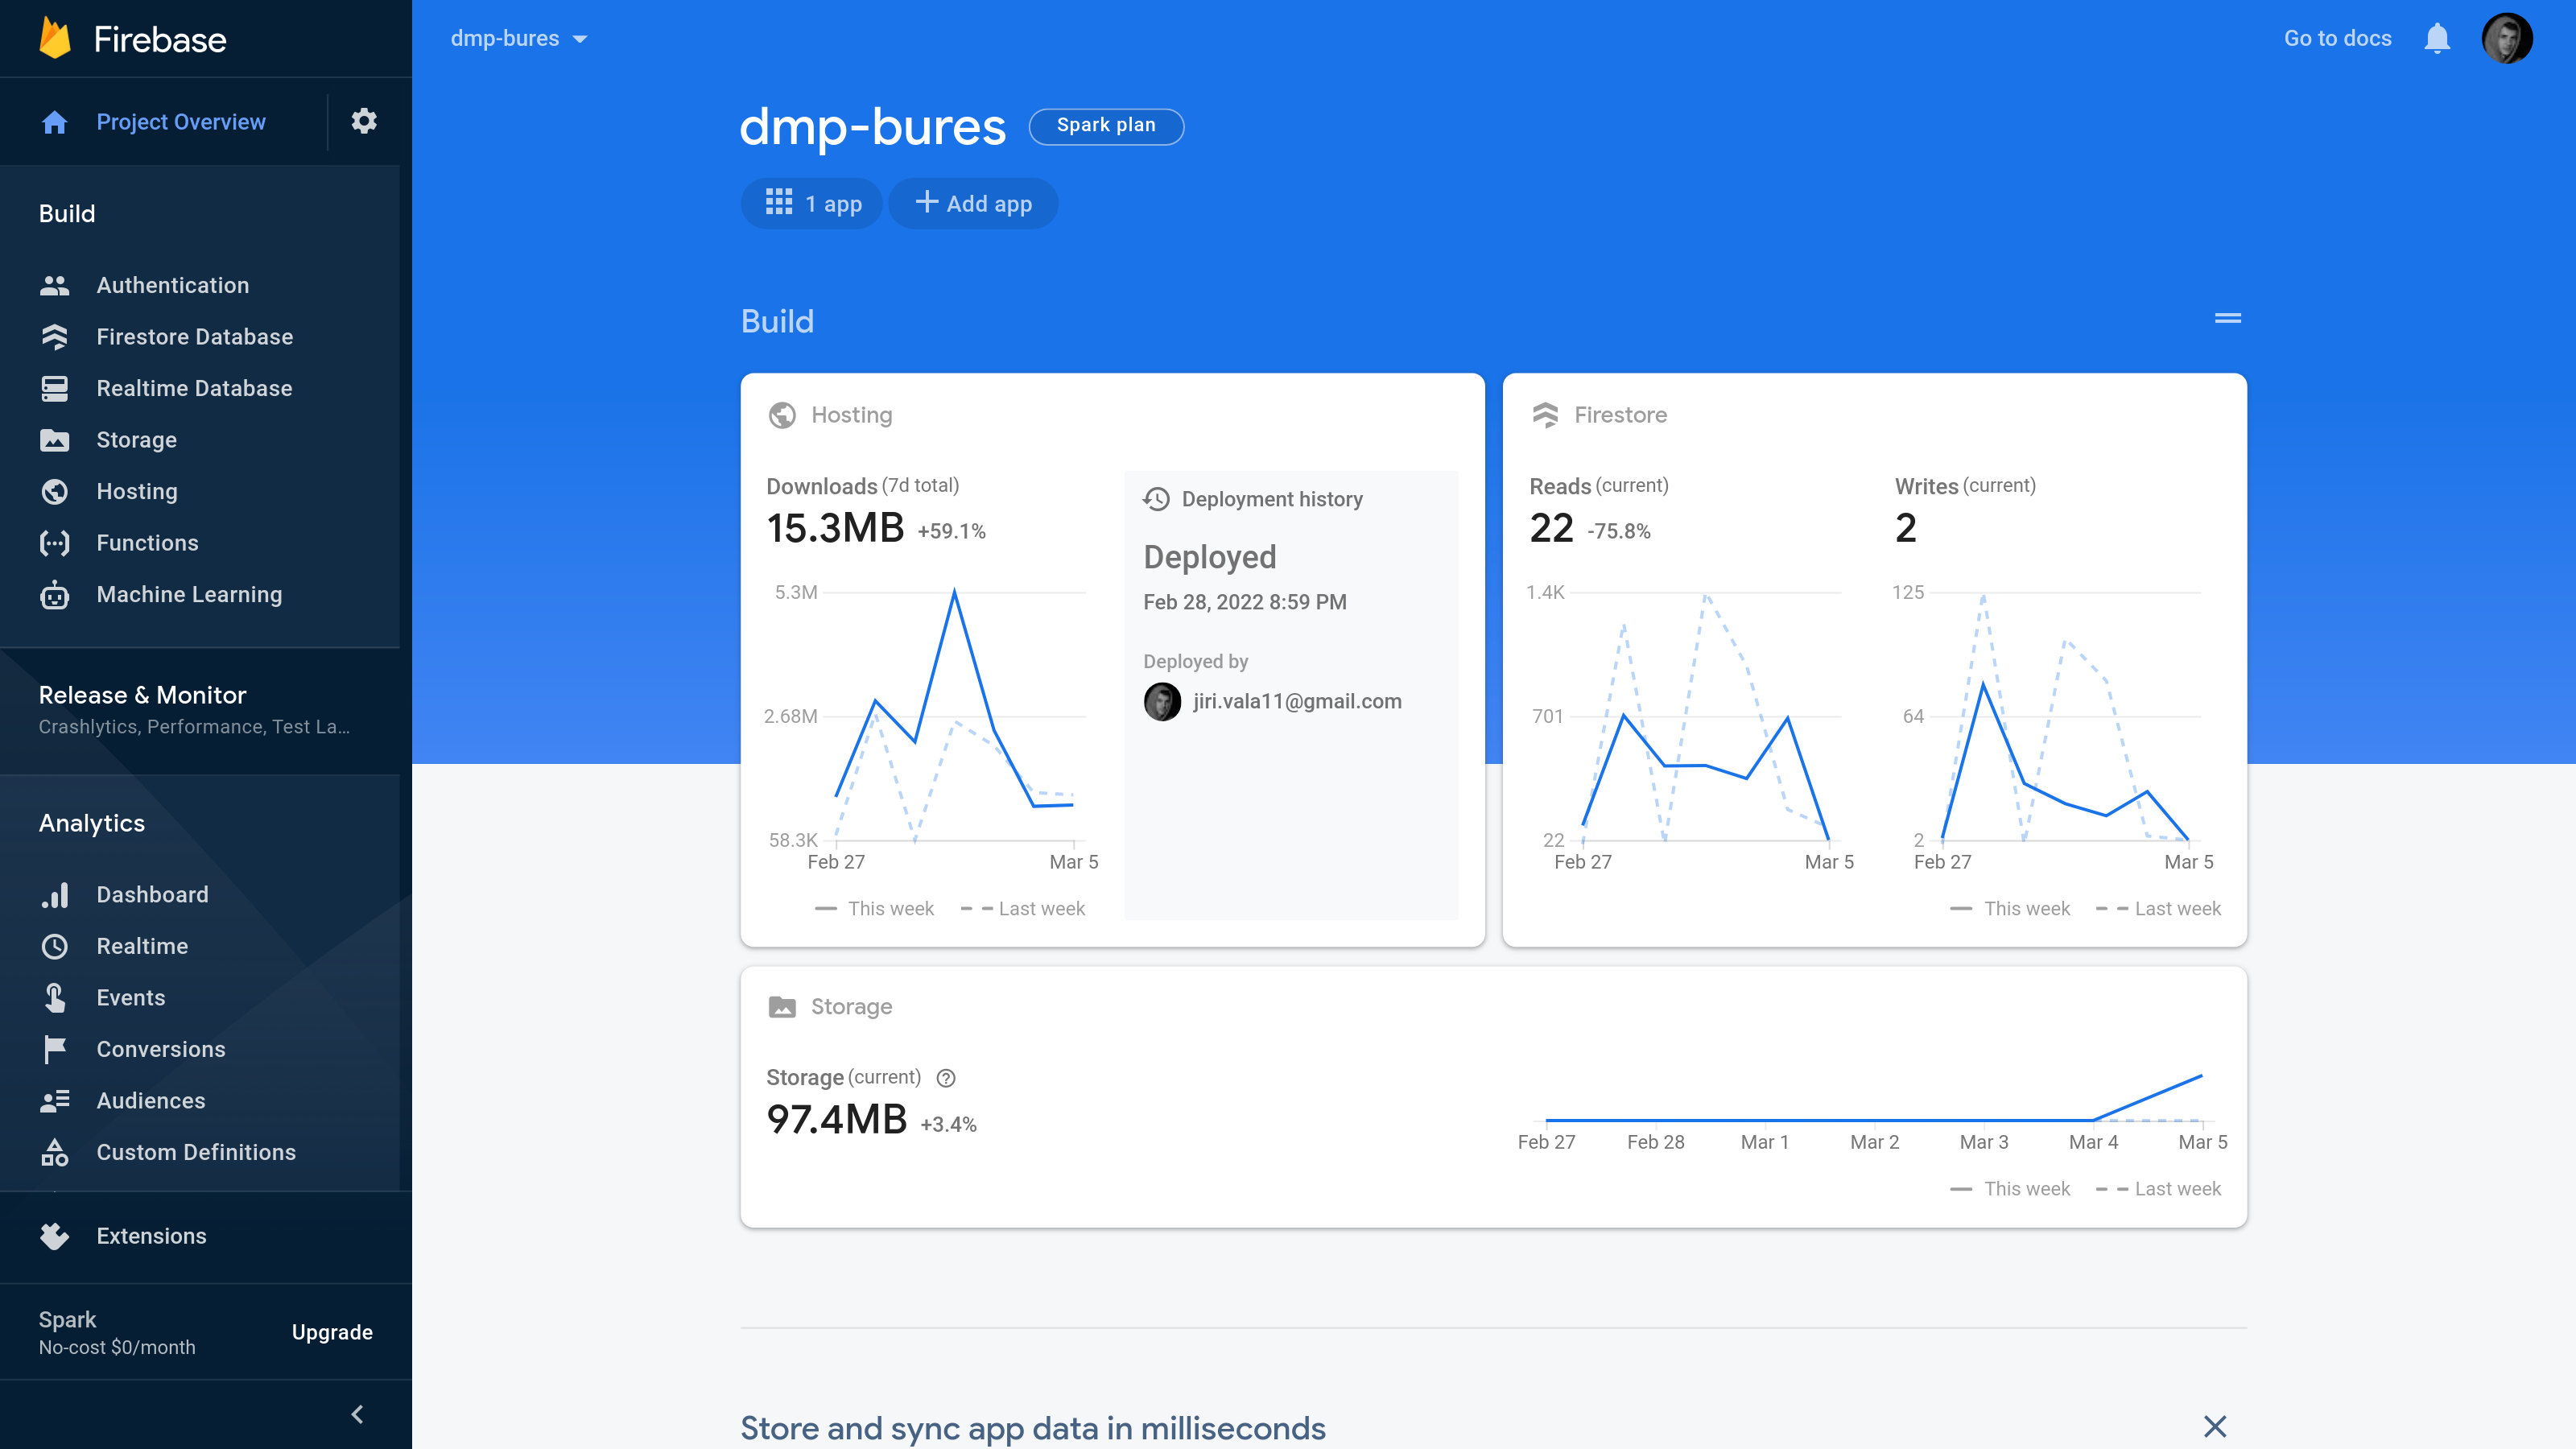
\includegraphics[width=\linewidth]{firebaseDash.png}
  \begin{center}
    Popis
  \end{center}
  \vspace*{0.5cm}
  Firestore je NO-SQL databáze, což znamená, že jednotlivé záznamy uchovává v datovém typu
  Objekt, což je key-value datový typ, který slouží pro jednoduché popisování parametru daného
  předmětu, například člověka. Pro mé účely (ukládání záznamů o jednotlivých albech a fotografiích)
  je naprosto dostačující, avšak jedinou nevýhodou je, že NO-SQL databáze neumí vytvářet relace
  mezi jednotlivými tabulkami, tudíž, když jsem chtěl vytvořit relaci mezi albem a jeho fotografiemi,
  musel jsem v albu vytvořit pole s názvem connectedImages a v něm uchovávat IDs všech těchto
  fotografií.

  \vspace*{0.5cm}
  \noindent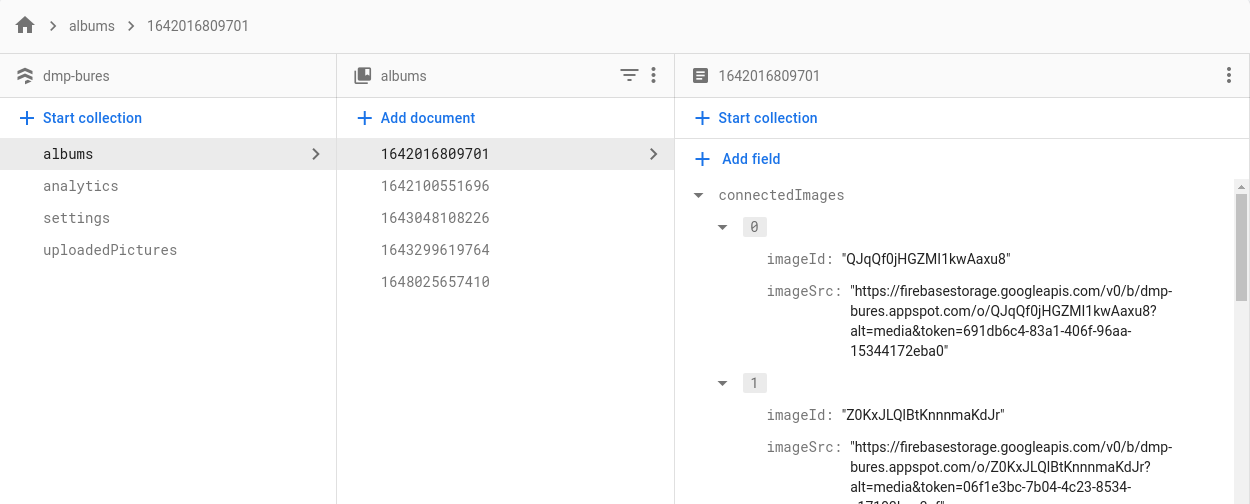
\includegraphics[width=\linewidth]{firestore.png}
  \begin{center}
    Popis
  \end{center}
  \vspace*{0.5cm}

  Cloud Storage je cloudové úložiště pro všechny typy souborů. Avšak vzhledem k tomu, že by pan
  fotograf měl nahrávat jen fotografie, ve scriptu, který řídí nahrávání nových fotografií je
  implementováno jednoduché ověření, zda li soubor, který se snaží nahrát, doopravdy je typu
  obrázku/fotky. Nicméně kdyby si to zákazník přál, jsem schopen implementovat i nahrávání
  souborů jiných, než fotografií.

  [helper functions codeblock]


  \chapter{Struktura projektu}
  REWRITE!!!!

  Projekt je rozdělen na dvě částí - komerční a školní (DMP). Co se týče části komerční, všechny
  služby okolo hostingu a databází bude zprostředkovávat Firebase, jelikož je to v rámci
  dlouhodobého hlediska nejjednodušší a hlavně nejlevnější řešení. Školní část (DMP) budu zcela
  spravovat já, tudíž mám pronajatý vlastní server, na kterém budu zprostředkovávat hosting a
  backend služby, nicméně všechna data budou poskytována a požadována z databází komerční
  části.
 
  \vspace*{0.5cm}
  \noindent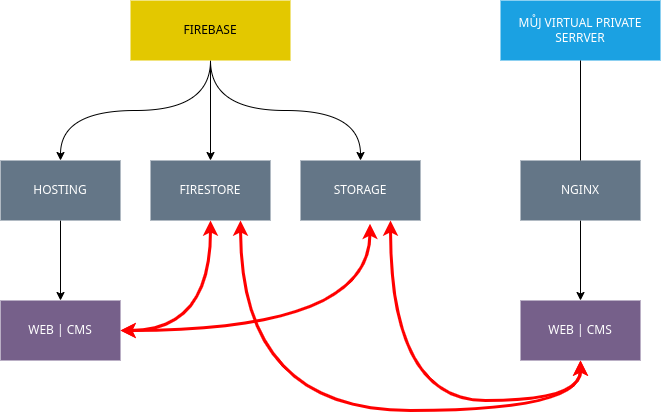
\includegraphics[width=\linewidth]{project_structure.png}
  \begin{center}
    Popis
  \end{center}
  \vspace*{0.5cm}


  \chapter{Průběh vývoje}
  Vývoj obou systémů, který započal dubnu roku 2021 jsem se snažil provádět co nejvíce agilně. To znamená,
  že se odehrával v takzvaných sprintech, kde jeden sprint je časový úsek pro implementaci a vyladění požadované změny.
  Nicméně častokrát se stalo, že jsme spolu se zákazníkem označili právě probíhající sprint za dokončený (já jsem implementoval změnu a zákazník ji označil za odpovídající), ale za pár dní mi 
  přišel email s tím, že se zákazníkovi tato změna nakonec nelíbí a chtěl by ji změnit, nicméně ikdyž se jedná lehce o kontraproduktivní chování, 
  je to zcela běžné i během vývoje mnohem větších a komplexnějších projektů a musí se s tímto počítat, proto je dobré, že je celý projekt modulární a není až tak složité implementovat změnu.
  
  \vspace*{0.5cm}
  \noindent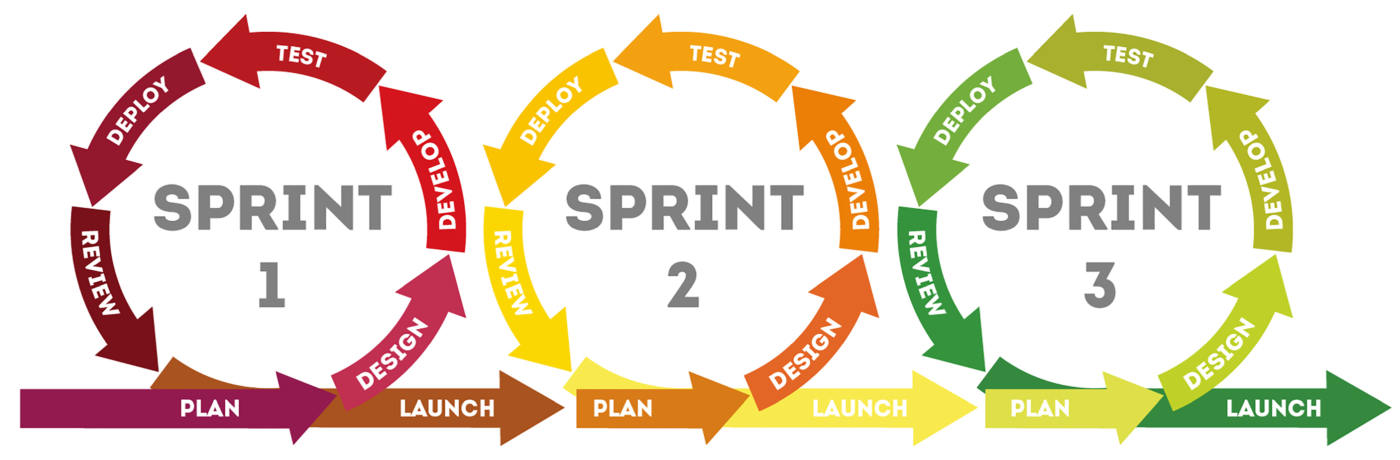
\includegraphics[width=\linewidth]{agile.png}
  \begin{center}
    Popis
  \end{center}
  \vspace*{0.5cm}
 
  Vývoj obou systémů začal nejprve ve vanilla Javascriptu, bez použítí jakéhokoliv frameworku, což
  se jevilo jako nejjednodušší řešení, jelikož jsem tehdy neuměl používat žádný framework. Čistý Javascript, je pro projekt, jako je webová stránka více než
  dostačující, nicméně vzhledem k modulárnosti a mnoha dalším vylepšením, které framework jako například Gatsby.js přidává, bych jej v případě, že bych měl vytvořit webovou stránku, použil.
  Nicméně se změnami a složitějšími funkcionalitami, které jsem postupně přidávala do administračního systému, se zdrojový kód začal jevit
  poměrně nepřehledným, a proto jsem se rozhodl, že jej refaktoruji do Reactu, který nejen zvýší celkovou rychlost a performance systému, ale také přehlednost struktury souborů a kódu,
  což se nakonec vyplatilo, protože nyní mám jasný přehled o tom, kde co je a jakým způsobem to funguje.

  \section{Komunikace se zákazníkem}

  \section{Organizace úkolů a změn k implementaci}

  \chapter{Webová prezentace}
  Webová prezentace bude panu fotografovi sloužit jako virtuální galerie fotek, aby lidé, které jeho
  tvorba zajímá, měli všechny jeho fotografie na "dosah ruky" a vzhledem k tehdejší koronavirové
  situaci je více než vhodné, aby nemuseli chodit přímo na výstavu.
  Samotná webová prezentace obsahuje přesně to, co obsahovala ta stávající, tedy, hlavní stránku,
  na které je jen galerie z alba "Hlavní", jelikož se jedná o fotografie, které se panu fotografovi líbí
  nejvíce a o kterých si myslí, že by mohly oslovit nejvíce lidí. Po kliknutí náhledovou fotografii se
  spustí galerie, která avšak nedovoluje rozkliknout informační box s více informacemi o dané
  fotografii.
  Data, které web používá k svému fungování nejsou dynamická, jelikož by to z principu fungování
  statické webové stránky nemělo smysl. Data se stahují z databáze ve chvíli, kdy uživatel přijde na
  stránku poprvé. To znamená, že pokud uživatel nahraje novou fotografii, změny na webu se
  projeví až ve chvíli, kdy uživatel stránku znovu načte.

  \vspace*{0.5cm}
  \noindent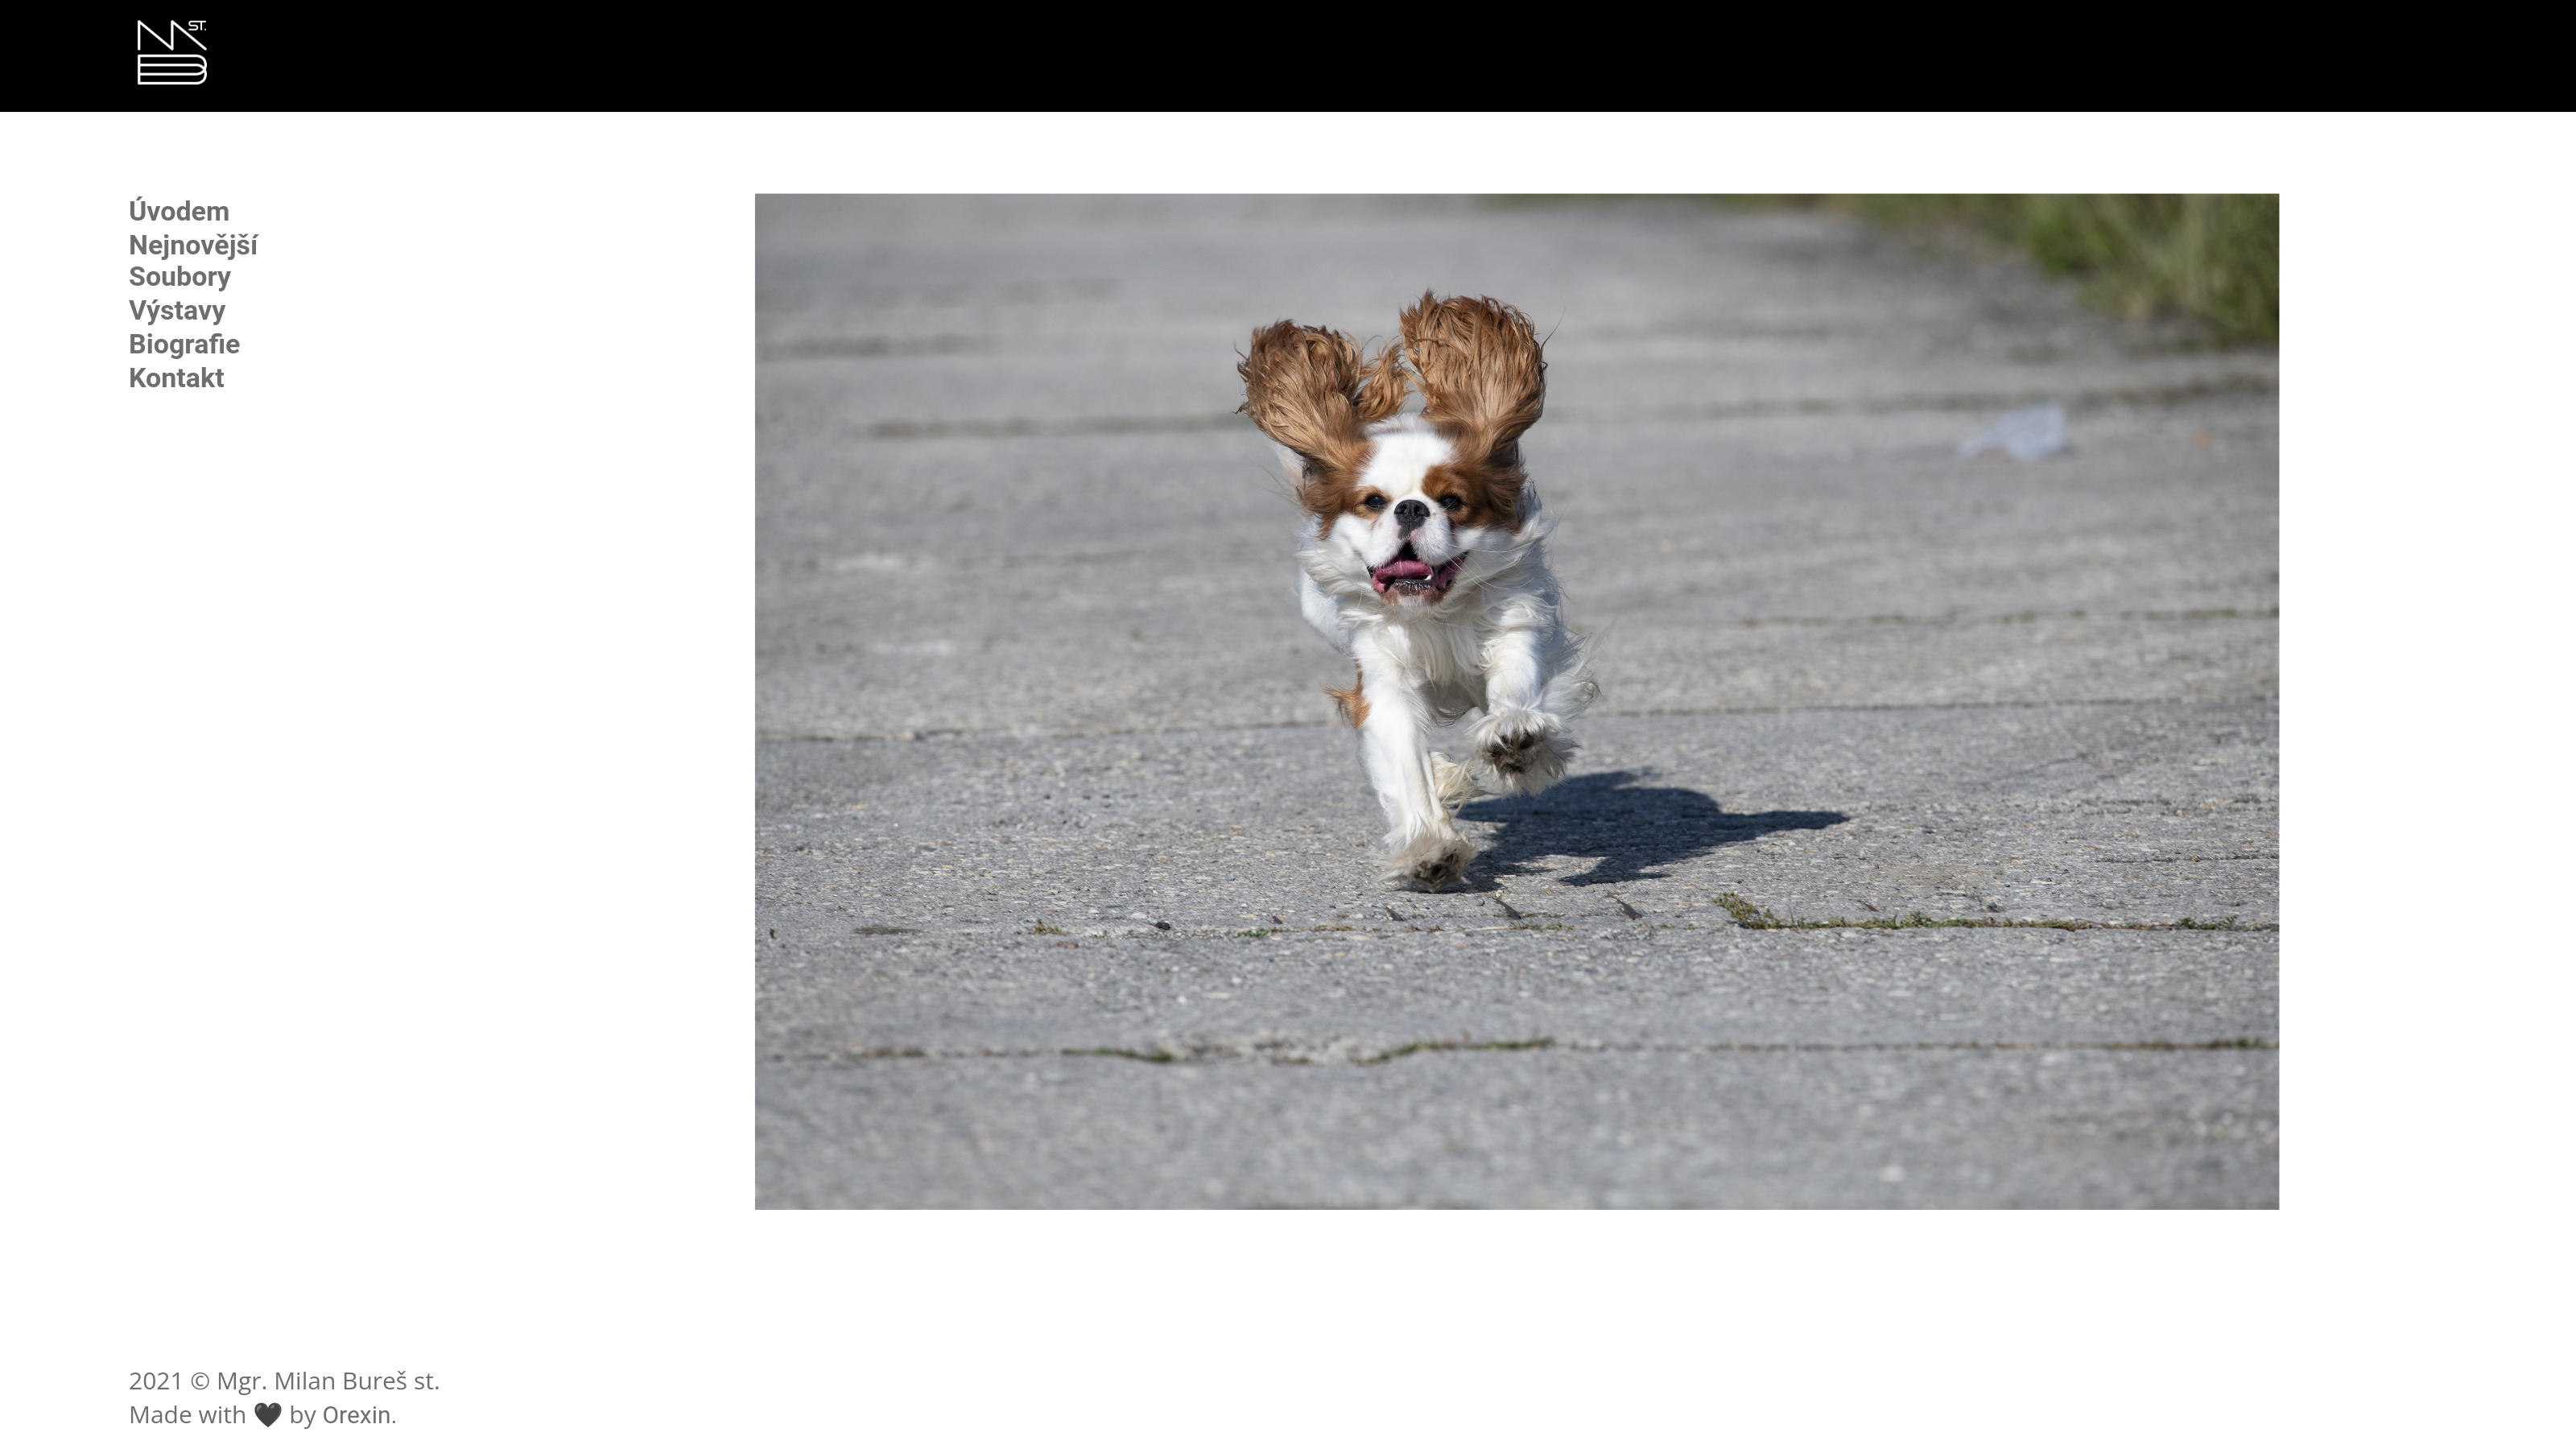
\includegraphics[width=\linewidth]{dmp-bures.png}
  \begin{center}
    Popis
  \end{center}
  \vspace*{0.5cm}

  Dále stránku "Úvodem", která slouží jako předmluva pro celý web, který má simulovat umělecké
  dílo spolu s jeho uměleckými fotografiemi. Tento text je samozřejmě editovatelný v
  administračním systému.
  Odkaz na stránku alba "Nejnovější". Nejedná se o, jak by se mohlo podle názvu zdát, album s
  fotografiemi, které byly nahrány nedávno, ale o fotografie, které byly nedávno vyfoceny, ostatní
  alba totiž mohou obsahovat i fotografie, které byly vyfoceny před rokem 2000. To znamená, že se
  jedná o výběr fotografií, které pan fotograf nedávno vyfotil a rozhodl se, že je bude sdílet. Při
  vývoji této podstránky jsem musel vymyslet systém, jakým budu fotografie na webu zobrazovat,
  jelikož si zákazník přál, aby místo galerie, která je použita u všech ostatních alb, byla použita
  tabulka s náhledy fotografií. Abych tohoto docílil, spolu se správnou pagination, musel jsem pole
  se všemi fotografiemi rozdělit na části po 6 fotografiích a poté je v těchto částech zobrazit na
  webu. Po kliknutí na náhled fotografie se však otevře galerie, jako u všech ostatních alb.
  
  \vspace*{0.5cm}
  \noindent\includegraphics[width=\linewidth]{album.png}
  \begin{center}
    Popis
  \end{center}
  \vspace*{0.5cm}

  Dropdown menu s odkazy na existující alba. Jelikož jsou alba dynamickými prvky v databázi, musel
  jsem vymyslet způsob, jakým budu vytvářet podstránky jednotlivých alb, nemohl jsem totiž ručně
  pro každé album vytvořit podstránku pokaždé, co ji uživatel administračního systému vytvoří.
  Implementoval jsem tedy algoritmus, který na základě id obsažené v URL linku alba vytáhne z
  databáze správný záznam o albu právě pomocí daného id.

  [show-correct-ulbum logic codeblock]
 
  Stránku "Výstavy", která obsahuje seznam všech výstav, na kterých pan fotograf kdy vystavoval
  své fotografie. Samozřejmě se jedná o editovatelný text.
  "Biografie" popisuje dosavadní život pana fotografa společně s jeho fotografií.
  
  V poslední řadě "Kontakt", kde lze najít veškeré kontaktní možnosti. Formulář, který podstránka
  obsahuje, bude pomocí Firebase Functions posílat email a push notifikaci panu fotografovi vždy,
  když mu někdo napíše email, aby se nikdy nestalo, že nebude vědět o tom, že mu někdo psal.
 
  \vspace*{0.5cm}
  \noindent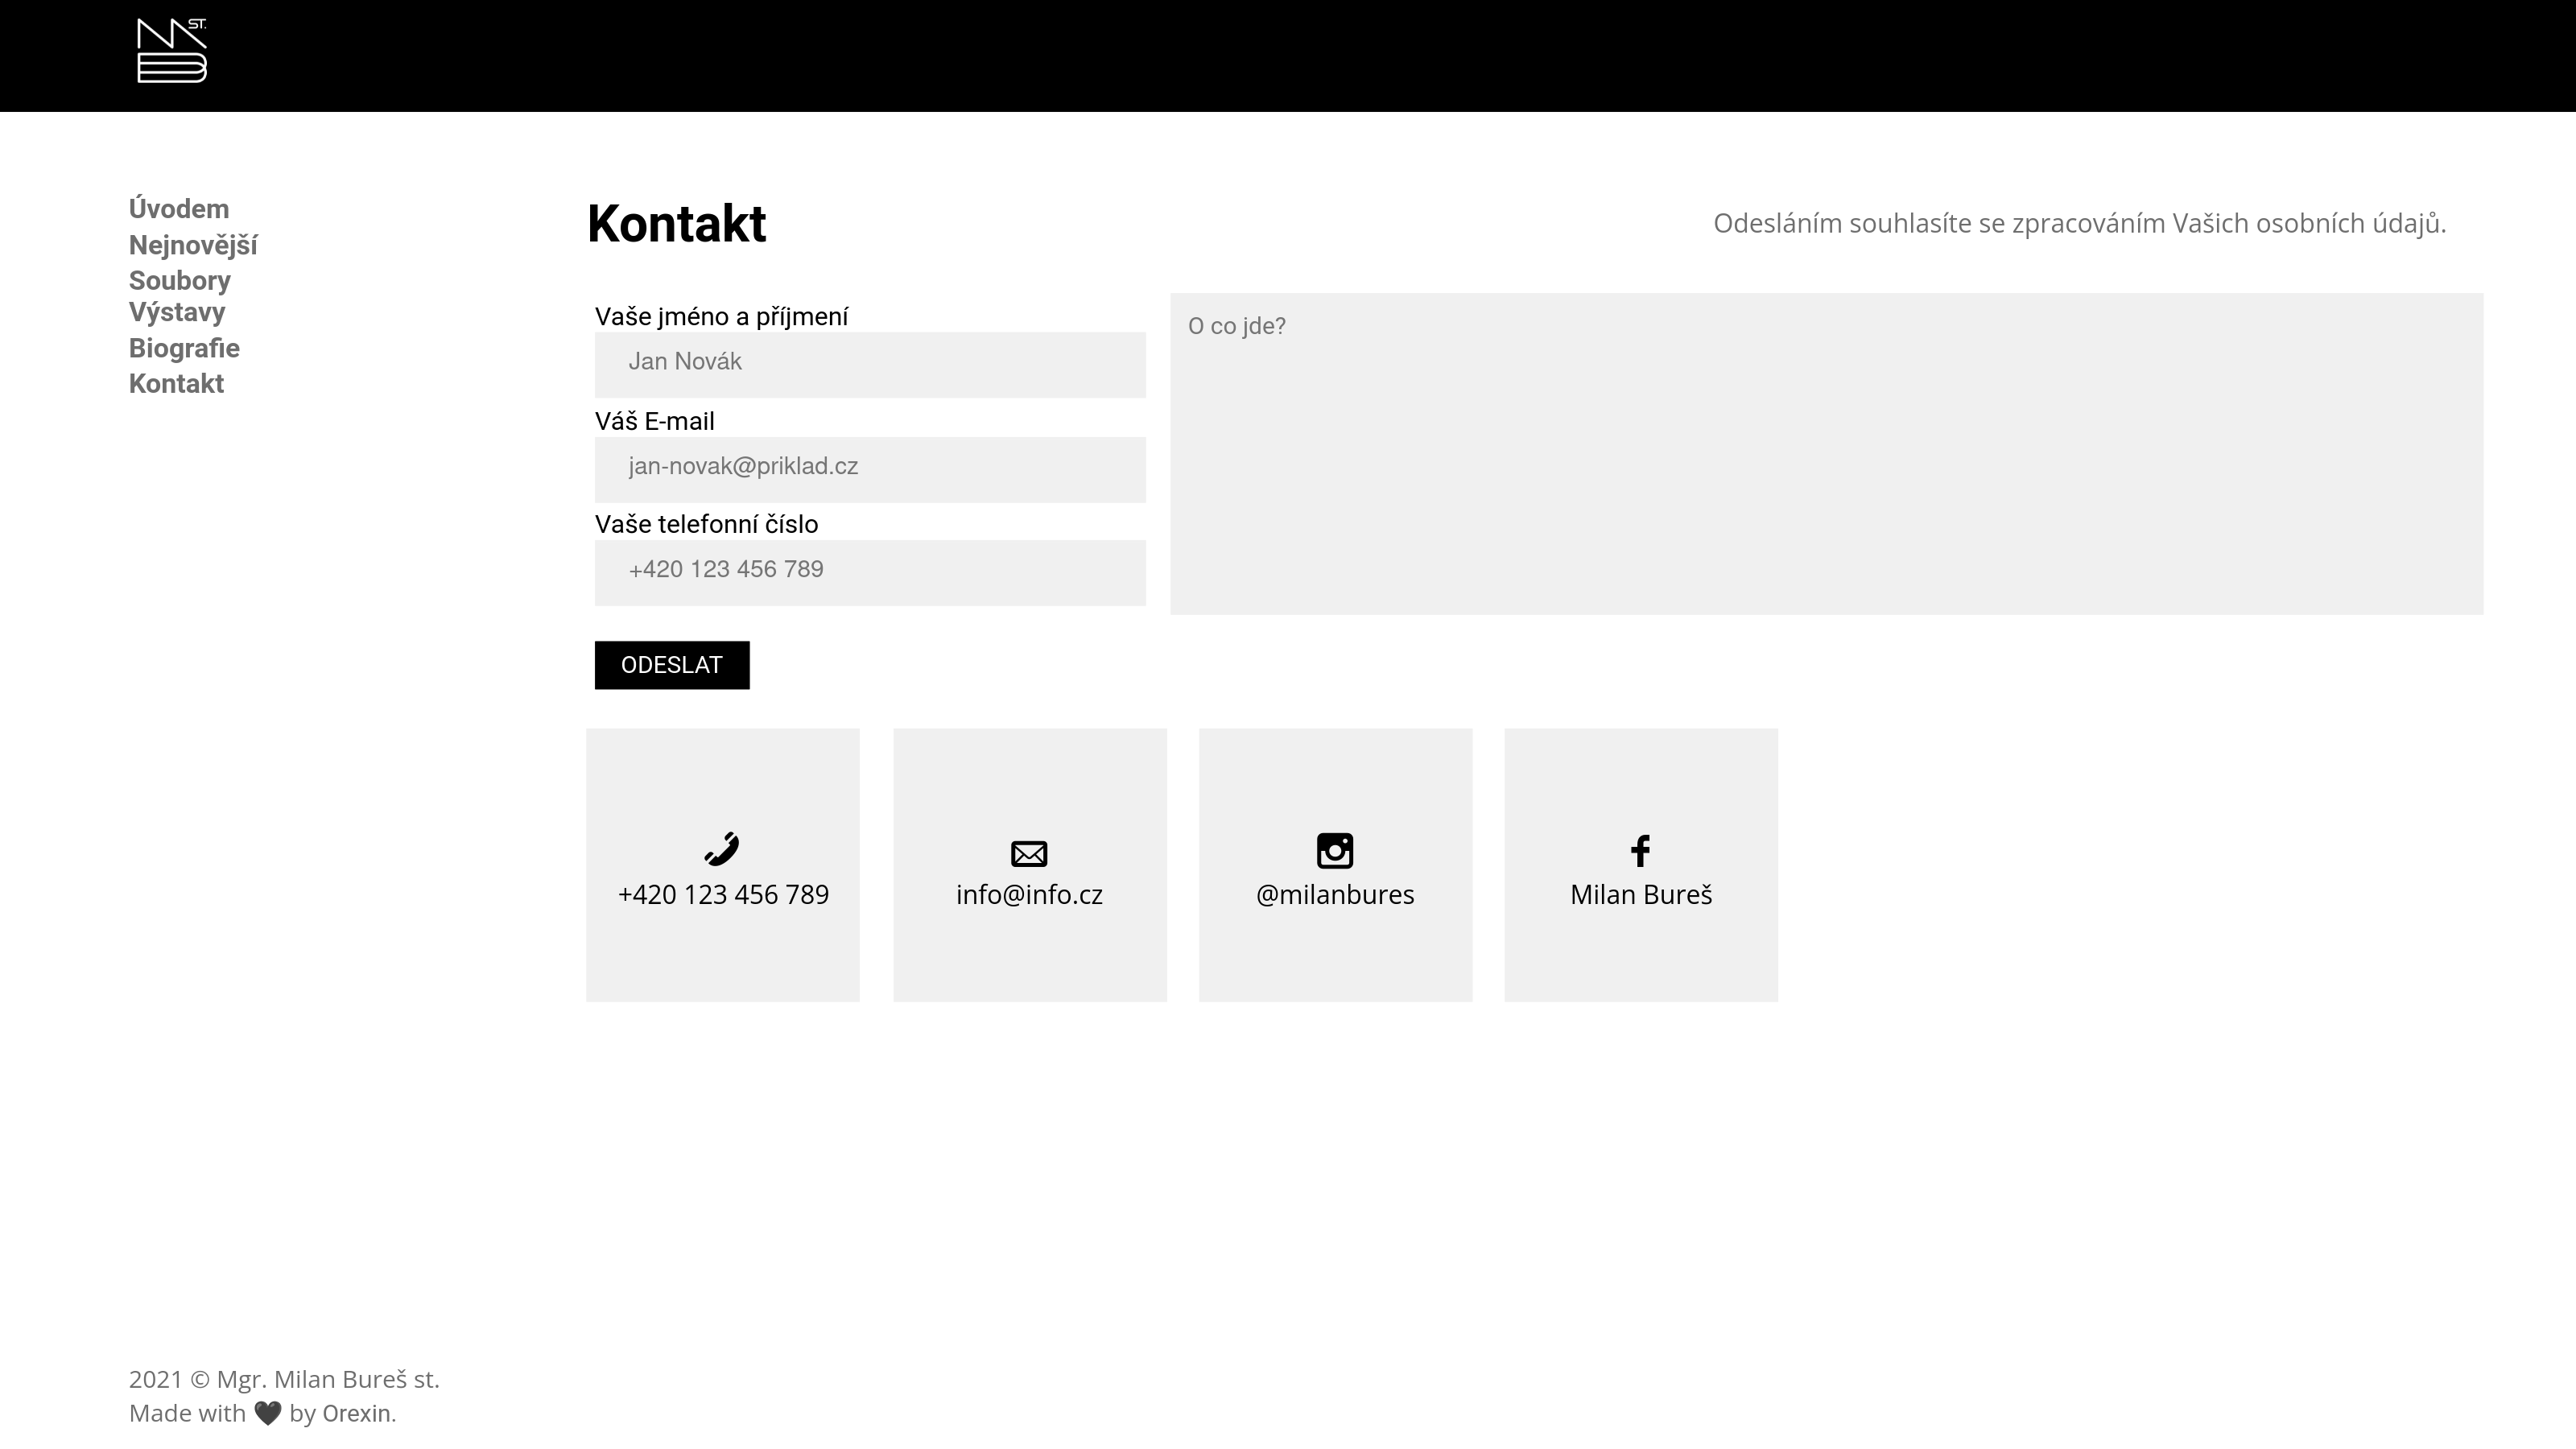
\includegraphics[width=\linewidth]{contact.png}
  \begin{center}
    Popis
  \end{center}
  \vspace*{0.5cm}

  Jelikož je webová prezentace napsána ve vanilla Javascriptu, v budoucnu mám v plánu ji přepsat
  pomocí frameworku Gatsby.js, který slouží pro generování statických HTML stránek za použítí
  React.js, což bude mít za následek nejen mnohonásobně jednodušší budoucí vývoj, ale také
  rychlejší načítací časy.

  \chapter{Administrační systém}
 
  Administrační systém je systém které zprostředkovává manipulaci s daty, které se objevují na
  dané webové stránce. Jednoduše řečeno, díky administračnímu systému je uživatel schopen své
  fotografie nahrávat, mazat, upravovat jejich název a popis, stejně tak jako uvidí, která z nich je
  nejvíce oblíbená na základě lajků a podobně. Dále administrační systém obsahuje funkcionalitu
  pro manipulaci s alby, do kterých bude uživatel své fotografie rozdělovat. Ty samozřejmě může
  obdobně vytvářet, mazat a upravovat jejich fotografický obsah. V neposlední řadě systém
  obsahuje i informační nástěnku, kde je velmi dobře vidět například kolik fotografií je v danou chvíli
  nahraných na webu a v jakých albech, kolik úložného prostoru jeho fotografie zabírají a nebo
  třeba seznam posledních nahraných fotografií, aby je nemusel hledat.

  \vspace*{0.5cm}
  \noindent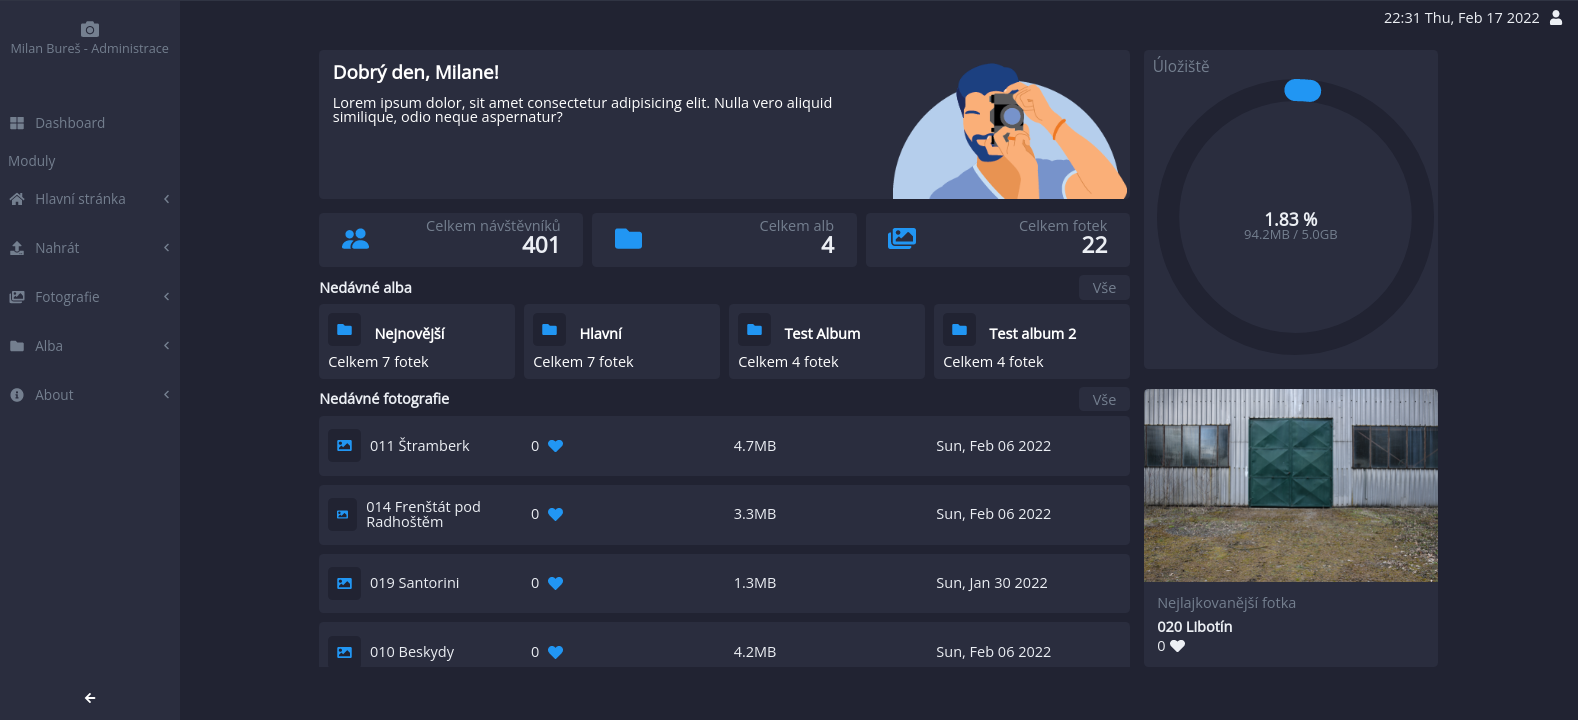
\includegraphics[width=\linewidth]{admin.png}
  \begin{center}
    Popis
  \end{center}
  \vspace*{0.5cm}

  Všechny data, se kterými uživatel pracuje, jsou zobrazována v reálném čase, což znamená, že
  pokud, například upraví název fotografie, tato změna se ihned projeví jak v samotném
  administračním systému, tak v databázi a tím pádem i na webové stránce.
  Díky Firebase Auth se do systému nedostane uživatel, který není autentifikovaný, tedy přihlášený.
  Prozatím celý autentifikační systém funguje za pomocí emailu a hesla, jelikož web spravuje jeden
  člověk a není potřeba, abych implementoval například autentifikaci pomocí Google či jiného již
  existujícího účtu.
  Celá aplikace je "obalená" v auth elemementu, který po úspěšném přihlášení (ověří se, zda
  uživatel existuje na Firebase Auth serveru) uchovává informace o přihlášeném uživateli a pokud
  záznam o tomto uživateli existuje, auth element jej pustí dál, jinak bude přesměrován zpět na
  přihlašovací obrazovku.
  Administrační systém obsahuje veškeré nástroje k tomu, aby uživatek mohl manipulovat s
  fotografiemi a alby, které nahraje a vytvoří. Po nahrání jedné či více fotografií se tyto fotografie
  objeví na podstránce "Fotografie" v přehledném seznamu. Kliknutím na jednotlivé fotografie se
  uživatel dostane na stránku pro manipulaci s jednotlivou fotografií, kde ji může přejmenovat,
  přidat popis, přiřadit do alba nebo ji z alba odstranit, a nebo fotografii odstranit úplně. Také lze
  vidět metadata fotografie, jako například kdy byla nahrána, či případně kolikrát ji návštěvníci
  webové prezentace udělili "lajk".

  \vspace*{0.5cm}
  \noindent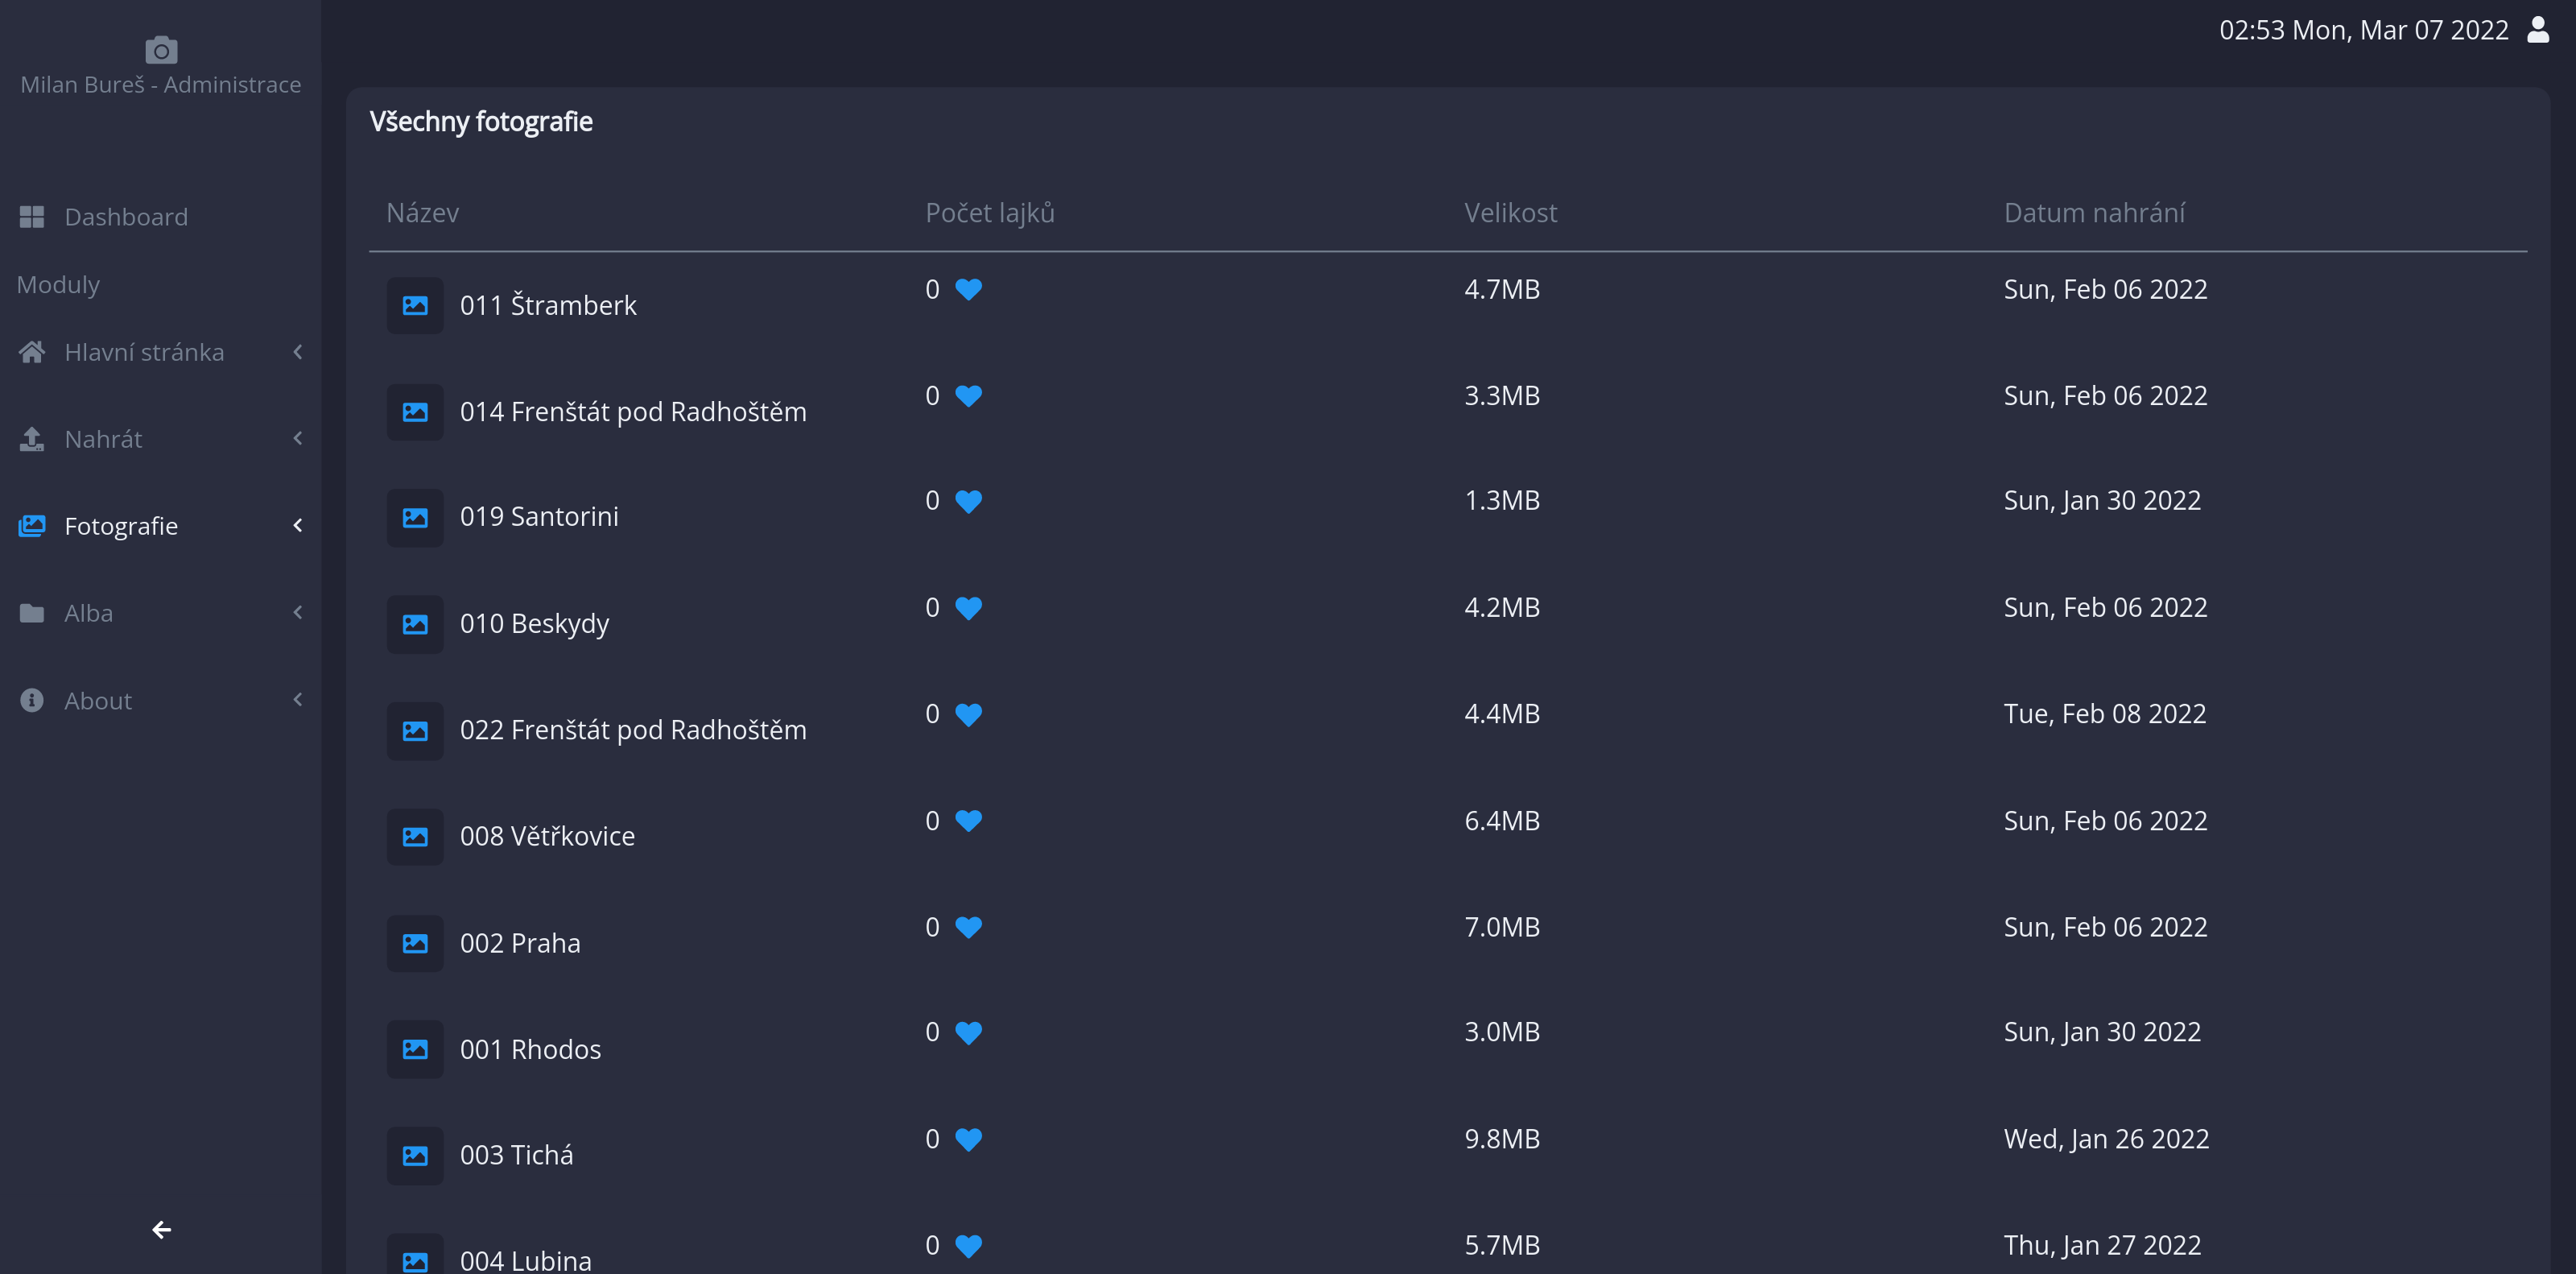
\includegraphics[width=\linewidth]{allPhotos.png}
  \begin{center}
    Popis
  \end{center}
  \vspace*{0.5cm}

  \vspace*{0.5cm}
  \noindent\includegraphics[width=\linewidth]{imageManipulator.png}
  \begin{center}
    Popis
  \end{center}
  \vspace*{0.5cm}

  \vspace*{0.5cm}
  \noindent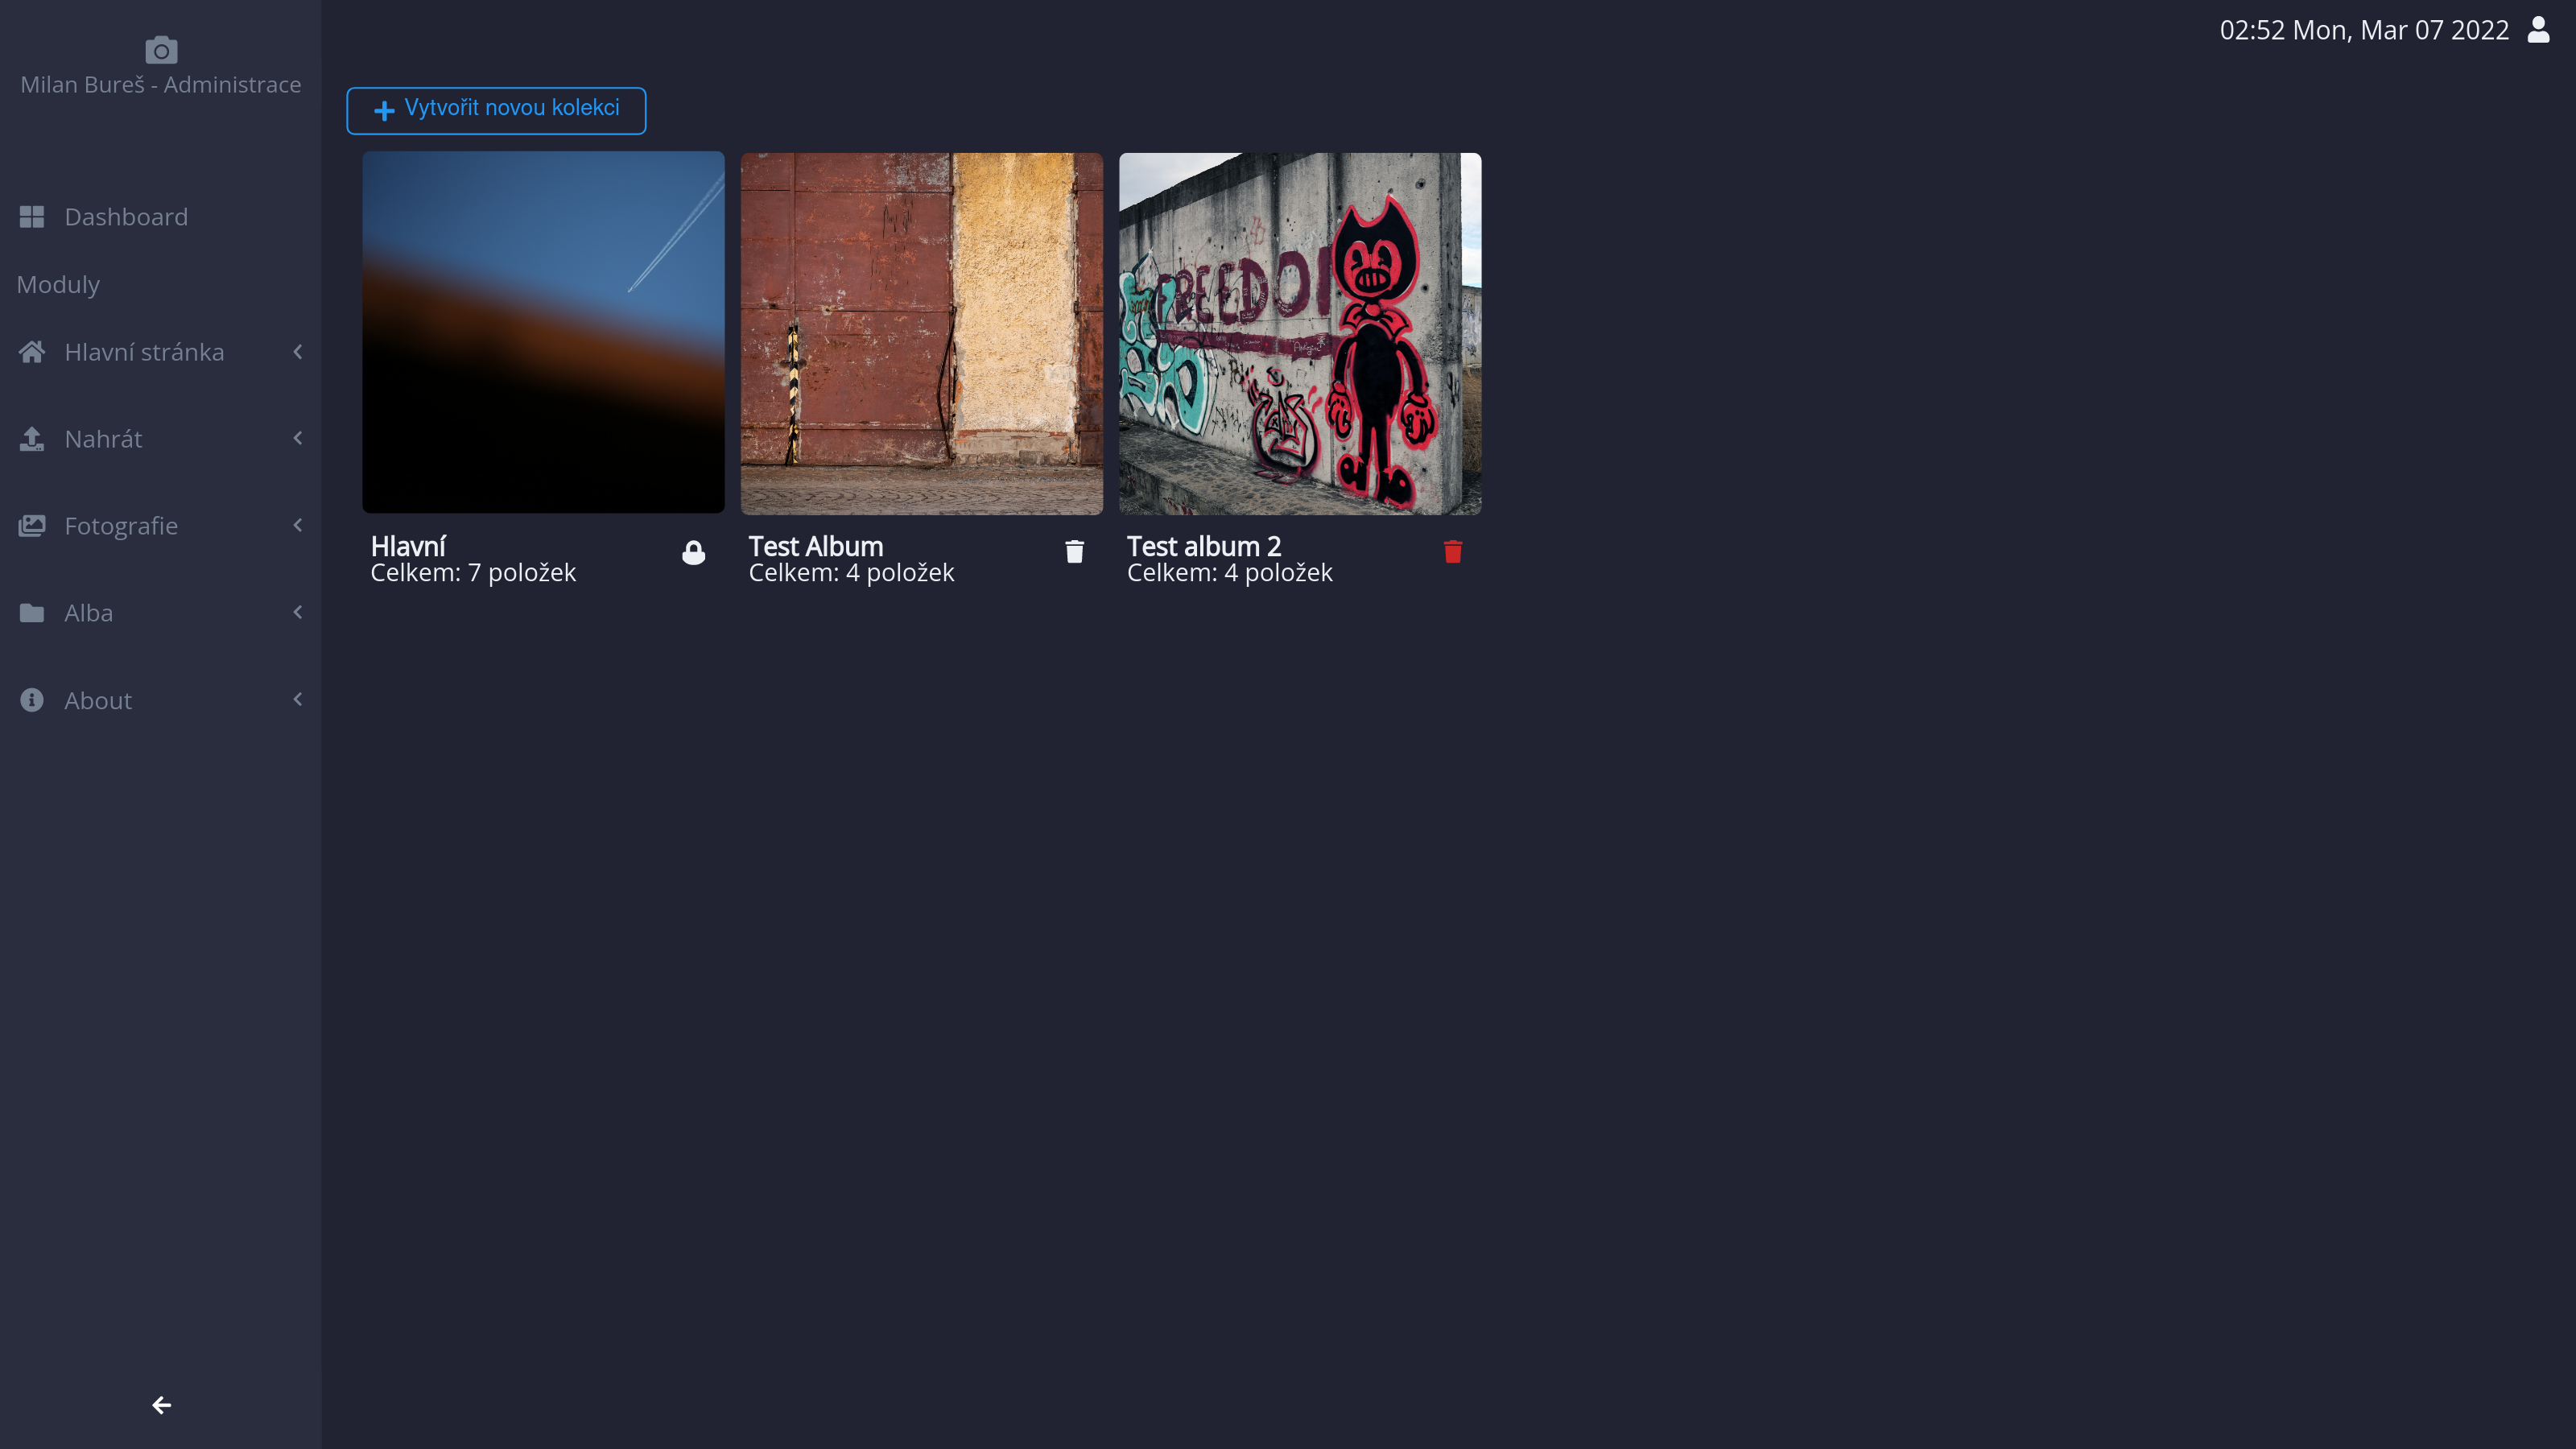
\includegraphics[width=\linewidth]{albums.png}
  \begin{center}
    Popis
  \end{center}
  \vspace*{0.5cm}
 
  \chapter{VPS - Virtual Private Server}
   Pro potřeby práce jsem si pronajal a nakonfiguroval vlastní server, který kopíruje veškeré funkcionality
   Firebase. Zajišťuje hosting pomocí softwarového webového serveru nginx, díky čemuž si na adrese VPS může
   zobrazit webovou stránku i modifikovat její obsah přes administrační systém. Kromě toho na VPS běží i Node.js backend server,
   díky kterému bude moct uživatel této instance projektu odesílat emaily panu fotografu bez použití email serveru třetí strany. 
   De-facto se jedná o druhou instanci komerčního projektu pro pana fotografa. 
  \section{VPS provideři}
  
  \begin{center}
    \begin{tabular}{|l|l|l|l|}
      \multicolumn{1}{c}{\bfseries Provider} & \multicolumn{1}{c}{\bfseries Cena} & \multicolumn{1}{c}{\bfseries Dalsi prop} & \multicolumn{1}{c}{\bfseries Dalsi prop} \\ \hline
      Digital Ocean & b & c & d \\ \hline
      Google Cloud Platform & b & c & d \\ \hline
      \end{tabular}
  \end{center}

  \section{Konfigurace VPS}
  \subsection{Operační systém GNU/Linux}
  V dnešní době je jako serverový operační systém nejvíce rozšířený GNU/Linux pro jeho
  minimalističnost a poměrně jednoduchou konfiguraci. Podle hostingtribunal.com až 96% serverů z
  1 milionu celosvětově nejpoužívanějších serverů používá Linux jako svůj operační systém a proto
  jsem se i já rozhodl použít Linux a nejen z toho důvodu, že jej dennodenně používám.
  \subsubsection{Debian 11}
  Jako cloud computing providera pro můj VPS jsem si vybral DigitalOcean, vzhledem k jeho ceně a
  celkové nabídce se jevil jako nejlepší. Původně jsem na svůj VPS chtěl nainstalovat Arch Linux,
  jelikož se jedná o Linuxovou distribuci, kterou dennodenně používám, nicméně má jednu velkou
  nevýhodu - nemá vlastní instalátor (i když nyní již existuje instalační script), což mě osobně při
  instalaci v domácích lokálních podmínkách vůbec nevadilo, ale v případě instalování Arche na VPS
  by to znamenalo, že bych musel mít vlastnoručně přizpůsobené ISO, které bych použil k instalaci,
  jelikož DIgitalOcean nenabízí Arch k nainstalování na jejich VPS, které nazývají Droplets.
  Volba tedy padla na Debian 11, jelikož je v jeho minimalistické instalaci poměrně "čistý" a tudíž
  neobsahuje zbytečné programy a podobně (bloatware). Vzhledem k tomu, že tento "počítač" bude
  sloužit jako server, není potřeba a je až zbytečné instalovat jakékoli desktopové prostředí GUI
  (Graphical User Interface), jelikož by to mělo nejen za následek zvýšení požadavků na výpočetní
  výkon serveru, což je nežádoucí, jelikož chceme, aby operační systém serveru zabíral co nejméně
  prostoru a prostředků, a zároveň celá konfigurace systému je proveditelná jen za pomoci
  příkazové řádky CLI (Command Line Interface). Na obrázku pod lze vidět, jak CLI-only Debian v idle
  stavu (stavu, kdy neprovádí žádné operace) zabírá na paměti RAM jen 89MB z dostupných 1GB,
  tedy necelých 10%.

  \vspace*{0.5cm}
  \noindent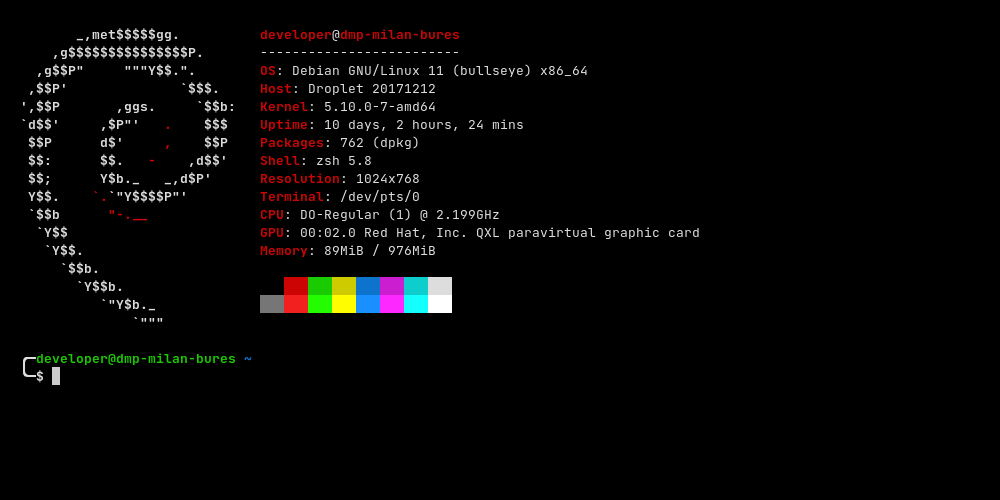
\includegraphics[width=\linewidth]{VPS.png}
  \begin{center}
    Popis
  \end{center}
  \vspace*{0.5cm}

  \subsection{Vytvoření developer uživatele}
  Tento uživatel bude využíván jako správce celého vývojového i produkčního prostředí a bude mít skoro stejná
  práva jako root. \\
  \begin{bash}
    useradd -m developer
    passwd developer
  \end{bash}
  Aby developer mohl naplno využívat systém, je potřeba, aby mohl používat sudo , které bylo díky
  Digital Ocean předinstalováno. Přídáme jej tedy do sudoers skupiny.\\
  \begin{bash}
    usermod -aG sudo developer
  \end{bash}
  A ověříme, že vše správně dopadlo:\\
  \begin{bash}
   su developer
   sudo -l
   [sudo]:
   User developer may run the following commands on dmp-milan-bures:
   (ALL : ALL) ALL
  \end{bash}


  \subsection{Konfigurace prostředí}
  \subsubsection{Shell}
  Vzhledem k tomu, že během práce s VPS používám git, který funguje na takzvaných větvích, je dobré vědět, se kterou větví právě pracuji.
  Proto nainstaluji jiný shell, který mi dovolí si jednoduše upravit příkazovou řádku.
  \begin{bash}
    sudo apt-get install zsh
  \end{bash}
  Zsh neboli Z-shell je mocný příkazový shell který odemyká mnoho možností ať už po stránce přizpůsobení vzhedu ale také vylepšení fukncí.
  V kombinaci s open-source projektem oh-my-zsh jsem schopen změnit nejen vzhled celé příkazové řádky, ale také přidat pluginy jako napřílad git, který mi, pokud se v aktuálním adresáři nachází .git soubor(soubor, který inicializuje složku jako git repozitář), zobrazí aktuálně zvolenou větev. Oh-my-zsh nainstaluji pomocí nástroje wget přímo z oh-my-zsh repozitáře na GitHubu, který poté spustí instalační script.
  
  \begin{bash}
    wget https://raw.github.com/ohmyzsh/ohmyzsh/master/tools/install.sh
    sh install.sh
  \end{bash}

  \subsubsection{Git a verzovací systém}
  Git je open-source nástroj pro správu verzí zdrojového kódu anebo jeho součástí vytvořený Linusem Torvaldsem. Jednoduše řečeno jedná se o software, který sleduje změny v souborech, aby pak měl uživatel/vývojář 
  větší přehled o tom, jaké změny provedl. V současnosti se git nejvíce používá pro kolaboraci mezi vývojáři na open-source ale i closed source projektech, jelikož git samotný je open-source, tudíž jej může kdokoliv využívat na svém interním serveru.
  Vzhledem k tomu, že z VPS nebudu pushovat žádné změny do remote repositáře, nebylo potřeba provádět žádnou pokročilejší konfiguraci a git stačí jen nainstalovat.
  \begin{bash}
    sudo apt-get install git
  \end{bash}
  Jediné, co jsem nakonfigurovat musel je zachování přihlašovacích údajů tak, aby se git nemusel pokaždé při každém pullu dotazovat na přihlašovací údaje k remote repository serveru, v mém případě ke Githubu.
  \begin{bash}
    git config --global credential.helper store
  \end{bash}
  \subsubsection{Node.js a NPM}
  Javascript samotný je spustitelný jen v prohlížeči, kde vetšinou plní funkci logického "mozku" webové stránky a provádí logické operace. Díky tomu avšak nemá moc jiného využití, což Node.js mění.
  Node.js je Javascript runtime, díky kterému můžeme spustit Javascriptový kód i mimo prohlížeč, jako například v příkazové řádce jako ostatní scriptovací ale i programovací jazyky, jako například Python nebo Java.
 
  Umožňuje nám API servery pro webové stránky i webové aplikace. 
  Jelikož je webová prezentace i administační systém serverless, není sám o sobě Node.js potřeba pro správnou funkčnost systému, ale vzhledem k faktu, že
  používím third-party knihovny a pluginy jako například webpack, musím Node.js nainstalovat. Tyto knihovny a další podpůrné programy lze nainstalovat pomocí takzvaného Node Package Manageru (Správce balíčků pro Node.js), neboli NPM.
  \begin{bash}
    sudo apt-get install nodejs npm
  \end{bash}
  Zjistíme verzi Node.js:
  \begin{bash}
    node -v
    [node]: v12.22.5
  \end{bash}
  A jelikož verze 12 není nejnovější, musím aktualizovat na nejnovější stable verzi, jinak by se totiž mohlo stát, že nějaká z dependencies, které v projektu používám, nebude se verzí 12 spolupracovat.
  \begin{bash}
    sudo npm i -g node
    sudo npm i -g npm
  \end{bash}
  A opět zkontrolujeme verzi Node.js:
  \begin{bash}
    node -v
    [node]: v16.14.0
  \end{bash}
  \subsubsection{Nginx}
  Nginx je open source softwarový webový server a load balancer, který se zaměřuje hlavně na co
  nejmenší konsumpci paměti a výkonu a skvěle zvládá velký nápor připojených zařížení.
  Nainstalujeme jej z Debian repositářů.
  \begin{bash}
    sudo apt-get install nginx
  \end{bash}
  A spustím pomocí systemctl.
  \begin{bash}
    sudo systemctl start nginx
  \end{bash}
  Nyní po úspěšném zapnutí nginx se VPS choová jako webový server a pokud v prohlížeči přejdu na adresu http://159.65.112.226/ (IP adresa VPS), zobrazí se přivítací obrazovka nginx, což indikuje, že je všechno správně nakonfigurováno a funkční. 
  \chapter{Závěr}
  Během vývoje tohoto projektu jsem se naučil mnoho nových věcí, které věřím, že mě v mém
  profesionálním životě posunuly dál, a jsem rád, že jsem si jako dlouhodobou maturitní práci
  vybral právě tento projekt. Mrzí mne však, že jsem začal pozdě s vývojem pomocí frameworku
  React.js, jelikož bych měl vývoj snazší a neztratil bych čas vyvíjením administračního systému ve
  vanilla Javascriptu a tím pádem bych se mohl soustředit na důležitější věci, než je opětovné
  vyvíjení systému, který jsem již jednou vytvořil.
 
  \chapter{Seznam použítého softwaru}
    \begin{enumerate}
      \item \textbf{Microsoft Visual Studio Code} - IDE použité k vývoji celého projektu.   
      \item \textbf{LaTeX} - 
      \item \textbf{Gimp} - 
      \item \textbf{Typora} - 
      \item \textbf{Gimp} -  
      \item \textbf{Git} -  
      \item \textbf{Github} -  
      \item \textbf{Stack Overflow} -  
      \item \textbf{????} - 
    \end{enumerate}
  \chapter{Seznam obrázků}
 
 
  \chapter{Citace}


\end{document}